%% START DUAL-BIRTH SUPPLEMENT
\chapter{Supplemental Material for Chapter~\ref{chap:dualbirth}}
\label{chap:dualbirth-sup}
\clearpage

\section{Theoretical Results}\label{sup:theory}\label{sup:sec:app-theory}
\subsection{Proofs}\label{sup:probdist}\label{sup:sec:app-theory-P2}
\label{sup:sec:cherries}
\label{sup:exp-bl}

\begin{theorem}\label{sup:thm:TRO}
Let $X$ be a random variable (r.v.) over ordered ranked tree shapes and distributed according to the dual-birth model with parameter $r=\la/\lb$. Then, 
\begin{equation}
\Pr(X=\TRO;n) = \frac{r^{\RBh-1}}{\prod_{i=1}^{n-2} \big((r-1)\LB{i}+i+1\big)}
\end{equation}
where $\RBh$ is the number of right leaves in $\TRO$ and $\LB{i}$ is the number of its left branches before node $i$.
\end{theorem}
\begin{proof}{Proof (sketch)}
Consider the intervals between consecutive birth events in $\TRO$, and denote each interval by the rank of its end node (e.g. Figure~\ref{fig:dualbirth-model}a). Because $\TRO$ is ordered, branches in the interval $i$ can be ordered from left to right (including the order of parents) and assigned an index between 1 and $i+1$. Two ordered ranked tree shapes are equal iff the index of the branch where node $i$ is born is identical in the two trees for all $i\in\NV$. Seeing that two identical ordered ranked shapes have this property is trivial. The opposite direction becomes clear if the nodes that give birth at point $i$ in the two trees are mapped together; the shapes become obviously equivalent (edges are the same), but also the ranking becomes the same. Finally, the ordering is the same because of identical left to right ordering. Let $\xi_i$ denote the event that the index of the branch on which node $i$ is born in $X$ is equal to the index of $i$ in $\TRO$. Then, $\Pr(X=\TRO)=\Pr(\cap_1^{n-2} \xi_i)$.

Birth on each branch is governed by a Poisson process with rate $\la$ and $\lb$ for left and right branches, respectively. Due to the memoryless property of the exponential distribution, the length of each branch before node $i-1$ has no bearing on subsequent birth events.

Thus, given $\LB{i}$ (the number of left branches in the interval $i$), the probability of $\xi_i$ does not depend on $\xi_1\ldots \xi_{i-1}$. Therefore, $\Pr(\cap_1^{n-2} \xi_i)=\prod_1^{n-2} \Pr(\xi_i;\LB{i})$. Also, the probability that any one of the $i+1$ competing independent Poisson processes (present on different branches of the interval $i$) results in the first event is simply the ratio of its rate to the sum of all rates. Thus,
$$\Pr(\xi_i;\LB{i})=\frac{\la(1-\SD_i)+\lb\SD_i}{\LB{i}\la+\big(i+1-\LB{i}\big)\lb}
=\frac{r(1-\SD_i)+\SD_i}{(r-1)\LB{i}+(i+1)}.$$
Multiplying $\Pr(\xi_i;\LB{i})$s and manipulations gives results.
\end{proof}

\begin{theorem}\label{sup:thm:cherr}
For a tree shape $Z$ generated by the dual-birth model with $r=\la/\lb$, let $C=\CH{Z}/n$ be an r.v.; then, 
\begin{align}\label{sup:eq:cherries}
\lim_{n\to\infty}\mathbb{E}(C) = \frac{\sqrt{r}}{1+r+\sqrt{r}}
\end{align}
\end{theorem}

\begin{corollary}\label{sup:cor:rbh}
For an r.v.\ $N_r$ capturing the number of right (i.e., active) leaves in tree shape $T$,
\begin{align}\label{sup:eq:nr}
\lim_{n\to\infty}\mathbb{E}(N_r) = \frac{\sqrt{r}}{1+\sqrt{r}}
\end{align}
\end{corollary}

\begin{proof}{Proof (sketch)}\
Our proof follows the approach of McKenzie and Steel~\cite{McKenzie2000}. We categorize the terminal branches (i.e., those incident on leaves) of an ordered tree shape into four types: right branch in a cherry (Right Cherry, or RC), right branch not in a cherry (Right Non-cherry, or RN), left branch in a cherry (Left Cherry, or LC), and left branch not in a cherry (Left Non-cherry, or LN). Note that the number of RC and LC branches must be equal (they could be potentially combined, but the discussions are more clear if we keep them separate). Suppose an urn includes four types of balls RC, RN, LC, and LN, respectively corresponding to these four types of branches. As the tree is evolving, each birth event adds a child to one of existing terminal branches. Moreover, the terminal branch to be used is chosen at random (but not uniformly) from the terminal branches available at that time point. After the birth, two new terminal branches are added and the original branch turns into an internal branch. Because of the memoryless property of our process, each birth event is equivalent to removing a ball from the urn and adding two balls back to the urn. To make matters slightly more complicated, a birth can also change the type of sibling branches that have not been removed (e.g. a non-cherry can be turned to a cherry). This can be modeled by removing a ball of one type and adding another ball of another type. In total, after each round, the number of added balls of each type can be potentially negative but the total number of new balls is a positive constant of 1; this kind of urn models are referred to as an \gls{EPU}.

For \glspl{EPU}, asymptotic central list theorems exist for the distribution of balls~\cite{Smythe1996}. Specifically, an \gls{EPU} with $k$ types can be described by a matrix $A_{k\times k}$, in which $A_{ij}$ gives the number of balls of type $j$ added when a ball of type $i$ was drawn. Under certain conditions~\cite{Smythe1996}, the number of balls of type $i$ out of $n$ total balls is asymptotically normally distributed with a mean of $n\lambda_1 v_i$, where $\lambda_1$ is the principal eigenvalue of $A$ and $v$ is its left eigenvector normalized to add up to one; more precisely, the number of all ball types asymptotically has a joint normal distribution. A birth in the dual-birth model can be described by
\begin{small}
$$
A'= 
\begin{matrix} 
RC: \\
RN: \\
LC: \\
LN:
\end{matrix}
\begin{bmatrix} 
0& 0&  0& 1 \\
1& -1&  1& 1 \\
0& 1&  0& 0 \\
1& 0&  1& -1 
\end{bmatrix}
$$ 
\end{small}

Let $p$ be the branch where the birth happens and let $s$ be the sister to $p$. Each birth always adds a new RC and a new LC branch, but depending on the type $p$
other changes will occur too. If $p$ is an RC branch, an RC branch ($p$) is removed, an RC and an LC are added, and $s$ changes from LC to LN. Thus, in total, we gain one LN; hence, the first row of $A'$. A similar logic gives the third row. For the second row, note that when $p$ is an RN type, we simply remove $p$, reducing the count of RN by one, and add an RC and an LC. A similar logic gives the last row. 

A further complexity is that not all branches will have an equal chance of splitting in the dual-birth model. Each left (or right) branch is selected with a probability proportional to $\la$ (or $\lb$). We account for this by replacing each left ball with $\la/\lambda=r/(r+1)$ balls and each right ball with $\lb/\lambda=1/(r+1)$ balls. Thus, we get

\begin{small}
$$
A= \frac{1}{r+1}
\begin{bmatrix} 
0& 0&  0& 1 \\
1& -1&  1& 0 \\
0& r&  0& 0 \\
r& 0&  r& -r 
\end{bmatrix}
$$ 
\end{small}

It can be checked that our \gls{EPU} satisfies the conditions of the \gls{EPU} central list theorem. The principle eigenvalue of $A$ is $\lambda_1=\frac{\sqrt{r}}{r+1}$, and \textit{a} left eigenvector is

\begin{small}
$$
v'= 
\begin{bmatrix}1+\sqrt{r}& r&  1+\sqrt{r}& \frac{1}{1+\sqrt{r}}
\end{bmatrix}$$
\end{small} 

The results immediately follow by computing $\lambda_1v'_1/\sum_1^4 v'_i$ for $\mathbb{E}(C)$ and $\lambda_1(v'_1+v'_2)/\sum_1^4 v'_i$ for $\mathbb{E}(N_r)$.
\end{proof}

\begin{theorem}
For a weighted tree shape $t$ generated by the dual-birth model with parameters $r$ and $\lambda$ conditioned on having $n$ leaves, let $\BL$ be an r.v.\ giving the length of a random branch in $t$; i.e., $\BL=\bl_I$ for $I\sim\mathcal{U}(1,n-2$). Then, 
\begin{align}\label{sup:eq:bl}
\lim_{n\to\infty}\mathbb{E}(\BL) \to \frac{1}{2\lambda}\left(\frac{r+1}{\sqrt{r}}\right)
\end{align}
\end{theorem}

\begin{proof}{Proof (sketch)}
It is constructive to think about the sampling strategy. First, an \textit{uncensored} tree is created with $n$ terminal branches but with varying depth for leaves. Half of the branches in this tree are drawn from the exponential distribution with rate $\la$ and the other half with rate $\lb$. Thus, the expected sum of branch lengths in the uncensored tree is $\frac{1}{2}(\frac{1}{\la}+\frac{1}{\lb})n$. We then cut $n-1$ branches. Because of the memoryless property of the exponential distribution, the expected length of the branches we cut from a tip is $1/\lb$ for right branches and $1/\la$ for left branches. By the proof of Corollary~\ref{cor:rbh}, the number of left and right branches are normally distributed with known expectation (Eq.~\ref{eq:bl}); thus,
$$
\mathbb{E}(\BL)=
\frac{1}{n}\left(\frac{n}{2\la}+\frac{n}{2\lb}-\left(\frac{\sqrt{r}}{1+\sqrt{r}}\frac{1}{\lb}+\frac{1}{1+\sqrt{r}}\frac{1}{\la}\right)(n-1)\right)
$$
which in limit gives the results. 
\end{proof}

\begin{lemma}\label{cherryparsimony}
For a tree shape $t$, the most parsimonious number of activation events is the minimum number of activation events possible, which is equal to the number of cherries in $t$.
\end{lemma}

\begin{proof}{Proof}
First, the most parsimonious number of activation events is the minimum number of activation events possible. As mentioned in the main paper, an activation event is a biological change, so a most parsimonious number of activation events would be one that minimizes the number of activation events. Note that, under the dual-birth model, the root node is considered an activation event.

Next, we prove that the minimum number of activation events possible is equal to the number of cherries in $t$. Let $N_t$ represent the minimum number of activation events possible for tree $t$, let $V_t$ denote the set of nodes in $t$, and let $a_v = 1$ if an activation event occurs on node $v$, otherwise $a_v = 0$. Under the dual-birth model, activation events only occur on nodes (i.e., not on edges), so $N_t = \sum_{v \in V}{a_v}$.

A node $v$ can have either 0 or 2 children. Under the dual-birth model, activation events occur when an inactive node gives birth to a new node, meaning activation events can only occur on internal nodes of $t$. Leaves that are active cannot undergo an activation event (by definition), and leaves that are inactive have not yet given birth, meaning they have not yet been activated. Therefore, for all leaves $f$, $a_f = 0$.

For an internal node $v$, there are three possible cases: both children of $v$ are leaves (i.e., $v$ is a cherry), one child is a leaf and the other is an internal node, or both children of $v$ are internal nodes.

If both children of $v$ are leaves (i.e., $v$ is a cherry), by definition, one child is active (and is therefore the propagation of $v$), and the other child is inactive. Therefore, either $v$ or an ancestor of $v$ must have undergone an activation event. Let $A_v$ denote the set of ancestors of node $v$. Because the dual-birth model does not allow deactivation, there can only be a single activation event in the lineage of an active node, meaning $a_v + \sum_{u \in A_v}{a_u} = 1$.

If one child of $v$ is an internal node and the other is a leaf, let $c$ denote the child that is an internal node. One of the descendants of $c$ must be a cherry. Therefore, there must be a cherry $u$ such that $v \in A_u$.

If both children of $v$ are internal nodes, by the same logic of the previous paragraph, $v$ must be the ancestor of at least two cherries: one for each of its internal node children.

Therefore, because each lineage of a cherry must have exactly 1 activation event, and because every internal node that is not a cherry much be in the lineage of a cherry, the minimum number of activation events possible would be a single activation event for each cherry's lineage. Therefore, the minimum number of activation events is equal to the number of cherries in $t$.
\end{proof}

\subsection{Set of all possible orderings:}
For $\TR \defeq(T,\RN)$, the set $\SDALL(\TR)$ of all possible orderings for $\TR$ (as shown in Figure~\ref{fig:dualbirth-model}c of the main paper) can be constructed recursively. For an internal node $u$ and its two children $\child{u}{1}$ and $\child{u}{2}$, let
\begin{equation*}
\SDALL'(\{u\}) =
\begin{cases}
\{\{(\child{u}{1},0),(\child{u}{2},1)\},\{(\child{u}{2},0),(\child{u}{1},1)\}\}
&  \text{if } \child{u}{1},\child{u}{2}\neq \leaf \\
\{\{(\child{u}{2},0)\},\{(\child{u}{2},1)\}\} 
& \text{if } \child{u}{1}= \leaf\\
\{\{(\child{u}{1},0)\},\{(\child{u}{1},1)\} \}
& \text{if } \child{u}{2}= \leaf\\
\{\{\}\} &  \text{if } \child{u}{1}=\child{u}{2}= \leaf 
\end{cases}
\end{equation*}
\begin{small}
and for two disjoint node sets $X$ and $Y$:
\begin{equation}\label{sup:eq:sdall}
\SDALL'(X\cup Y) = \{\SD_X \cup \SD_Y| (\SD_X,\SD_Y ) \in \SDALL'(X) \times \SDALL'(Y)\}.
\end{equation}
\end{small}
Then, $\SDALL(\TR)=\{\SD_X\cup\{(r,1)\} | \SD_X\in \SDALL'(V)\}$ where $r$ is the root.

\section{Supplementary methods}
\subsection{Simulation setup}\label{sup:simsetup}
\subsubsection{Motivation of Default Parameters}\label{sup:simsetup-mot}
The default value of $n = 1,000$ (which is used for all trees in all experiments) is chosen because it is large enough to observe changes in tree shape resulting from tweaking the other parameters, yet it is small enough that simulations and subsequent tree inferences remain computationally tractable. The default values for the alignment simulation parameters, including \gls{GTR} parameters, are chosen based on ML estimates from of the \textit{Alu}  tree as computed by FastTree-2 (see Section~\ref{sec:dualbirth-human-alu-analyses}).

The default value of $r=10^{-2}$ is chosen because $r=1$ is equivalent to the Yule model and $r=10^{-4}$ results in an almost fully ladder-like tree, so $r=10^{-2}$ serves as an intermediate. The default value of $\lambda=169.328$ is chosen because the best estimate of the average branch length of the \textit{Alu} tree is 0.029824, which can be used with the default value of $r=10^{-2}$ to find $\lambda$ (Eq.~\ref{eq:bl}). $k=300$ is chosen to match the length of \textit{Alu}.

The default value of ultrametricity deviation gamma distribution rate $\alpha=29.518$ is chosen by first rooting the best estimate of the \textit{Alu} tree on the MRCA of 7SLRNA sequences, which we assume is the outgroup of the \textit{Alu} elements~\cite{Deininger2011}. Then, root-to-tip distances are computed and are normalized by the distribution average. A gamma distribution is then fit on the resulting distribution with the constraint that the distribution's rate and shape must be equal.

\subsubsection{Data generation}
To generate ``true trees,'' we use our implementation of the generative process of the dual-birth model, which takes three parameters: $\la$, $\lb$, and $n$. We then deviate each tree from ultrametricity by multiplying each branch of the tree by a multiplier sampled from a gamma distribution with shape and rate both set to some parameter $\alpha$ (so as to keep the expected value of the distribution equal to 1, and as a result, keep the average branch lengths of the trees constant). We then simulate a multiple sequence alignment with no indels according to the \gls{GTR}+$\Gamma$ model using INDELible.

We have a series of ``experiments,'' where we start with a default set of parameters and then deviate one parameter at a time.

\begin{itemize}
\item \textbf{INDELible Parameters (Global)}
\begin{itemize}
\item \gls{GTR} Frequencies: 0.2922 0.2319 0.2401 0.2358
\item \gls{GTR} Rates (ac ag at cg ct gt): 0.8896 2.9860 0.8858 1.0657 3.8775 1.0000
\item $\alpha = 5.256$
\end{itemize}

\item \textbf{Default Parameters (param-00)}
\begin{itemize}
\item $n = 1000$ (Global)
\item $r = 10^{-2}$
\item $\la = 1.6765100539857060$
\item $\lb = 167.65100539857060$
\item Ultrametricity Gamma Distribution Parameter $\alpha = 29.518173529892621$
\item Sequence Length = 300
\end{itemize}

\item \textbf{Experiment 1 (Changing $r$) (Constant Average Branch Length)}
\begin{itemize}
\item param-04: $r = 10^{-4}$, $\la = 0.16765100539857060$, $\lb = 1676.5100539857060$
\item param-03: $r = 10^{-3}$, $\la = 0.53015902907666816$, $\lb = 530.15902907666816$
\item param-00: $r = 10^{-2}$, $\la = 1.6765100539857060$, $\lb = 167.65100539857060$
\item param-02: $r = 10^{-1}$, $\la = 5.3015902907666816$, $\lb = 53.015902907666816$
\item param-01: $r = 10^{0}$, $\la = 16.765100539857060$, $\lb = 16.765100539857060$
\end{itemize}

\item \textbf{Experiment 2 (Changing Model of DNA Evolution)}
\begin{itemize}
\item param-00: JC69
\item param-00: K80
\item param-00: HKY85
\item param-00: GTRCAT
\item param-00: \gls{GTR}+$\Gamma$
\end{itemize}

\item \textbf{Experiment 3 (Changing $\lambda$)}
\begin{itemize}
\item param-05: $\la = 0.33530201079714$, $\lb = 33.53020107971412$
\item param-06: $\la = 0.83825502699285$, $\lb = 83.8255026992853$
\item param-00: $\la = 1.6765100539857060$, $\lb = 167.65100539857060$
\item param-07: $\la = 3.35302010797141$, $\lb = 335.3020107971412$
\item param-08: $\la = 8.38255026992853$, $\lb = 838.255026992853$
\end{itemize}

\item \textbf{Experiment 4 (Changing Sequence Length)}
\begin{itemize}
\item param-09: Sequence Length = 50
\item param-10: Sequence Length = 100
\item param-11: Sequence Length = 200
\item param-00: Sequence Length = 300
\item param-12: Sequence Length = 600
\item param-13: Sequence Length = 1200
\item param-14: Sequence Length = 2400
\item param-15: Sequence Length = 4,800
\end{itemize}

\item \textbf{Experiment 5 (Changing Number of Leaves $n$)}
\begin{itemize}
\item param-25: $n = 25$
\item param-26: $n = 50$
\item param-27: $n = 250$
\item param-28: $n = 500$
\item param-00: $n = 1000$
\item param-29: $n = 2000$
\item param-30: $n = 4000$
\end{itemize}

\item \textbf{Experiment 6 (Changing Ultrametricity Gamma Distribution Parameter $\alpha$)}
\begin{itemize}
\item param-16: $\alpha = 2.95181735298926$
\item param-17: $\alpha = 5.90363470597852$
\item param-00: $\alpha = 29.518173529892621$
\item param-18: $\alpha = 147.590867649463$
\item param-19: $\alpha = 295.181735298926$
\item param-20: $\alpha = 9999999999999999$ (i.e., $\infty$)
\end{itemize}
\end{itemize}

\subsubsection{Methods}
For each alignment created by INDELible (one alignment per ``true tree''), we use FastTree-2 and RAxML to infer a tree using the \gls{GTR}+$\Gamma$ model. We run RAxML a second time on the trees outputted by RAxML in order to compute branch support values. We then estimate cherries using the method described in Section~\ref{sec:dualbirth-paramest}.
\begin{itemize}
\item \textbf{FastTree~2:} \texttt{fasttree -nt -gtr -gamma < SEQS}
\begin{itemize}
\item \texttt{-nt:} Alignment contains nucleotide sequences
\item \texttt{-gtr:} Use \gls{GTR} model
\item \texttt{-gamma:} Rescale tree's branch lengths to optimize Gamma20 likelihood
\item \texttt{SEQS:} INDELible multiple sequence alignment (FASTA)
\end{itemize}

\item \textbf{Initial RAxML (Tree Inference):} \texttt{raxmlHPC -s SEQS -m GTRGAMMA\\-n OUT -p \$RANDOM}
\begin{itemize}
\item \texttt{-s SEQS:} Specify the sequence alignment file to be \texttt{SEQS} (FASTA)
\item \texttt{-m GTRGAMMA:} Use the \gls{GTR}+$\Gamma$ model
\item \texttt{-n OUT:} Specify output project name to be \texttt{OUT}
\item \texttt{-p \$RANDOM:} Use a random number as the seed
\end{itemize}

\item \textbf{Final RAxML (Branch Support):} \texttt{raxmlHPC -f J -p \$RANDOM\\-m GTRGAMMA -s SEQS -t TREE -n OUT}
\begin{itemize}
\item \texttt{-f J:} Compute SH-like support values on the given tree
\item \texttt{-p \$RANDOM:} Use a random number as the seed
\item \texttt{-m GTRGAMMA:} Use the \gls{GTR}+$\Gamma$ model
\item \texttt{-s SEQS:} Specify the sequence alignment fileto be \texttt{SEQS} (FASTA)
\item \texttt{-t TREE:} Specify the input tree (from ``Initial RAxML'' step)
\item \texttt{-n OUT:} Specify output project name to be \texttt{OUT}
\end{itemize}

\item \textbf{Cherry Estimation:} \texttt{estimate-cherries.sh TREE THRESHOLD}
\begin{itemize}
\item \texttt{TREE:} Tree for which to estimate cherries
\item \texttt{THRESHOLD:} Branch support threshold to use
\end{itemize}
\end{itemize}

\subsubsection{Error measurement}
We measure the accuracy of inferred tree topology using the \gls{RF} distance as well as the \gls{MS} metric.

\begin{itemize}
\item \textbf{RF Computation:} \texttt{echo \$(echo -n '(' \&\&\\echo -n `compareTrees.missingBranch TRUE INFERRED | cut -d' ' -f3` \&\&\\echo -n ' + ' \&\&\\echo -n `compareTrees.missingBranch INFERRED TRUE | cut -d' ' -f3` \&\&\\echo -n ') / 2') | bc -l}
\begin{itemize}
\item \texttt{TRUE:} ``True tree'' simulated by our dual-birth simulation tool
\item \texttt{INFERRED:} Inferred tree (from either FastTree~2 or RAxML)
\item \texttt{compareTrees.missingBranch:} Tool to compute missing branch rate (FN) between two trees
\item First compute FN of \texttt{INFERRED} with respect to \texttt{TRUE}
\item Then compute FN of \texttt{TRUE} with respect to \texttt{INFERRED}
\item Average these two FN values to compute the RF metric
\end{itemize}

\item \textbf{\gls{MS} Computation:} \texttt{TreeCmp.jar -r TRUE -d ms -i INFERRED}
\begin{itemize}
\item \texttt{TRUE:} ``True tree'' simulated by our dual-birth simulation tool
\item \texttt{INFERRED:} Inferred tree (from either FastTree~2 or RAxML)
\item \texttt{TreeCmp.jar:} Tool used to compute MS metric~\cite{Bogdanowicz2012}
\item \texttt{-r TRUE:} Specify \texttt{TRUE} to be the reference tree
\item \texttt{-d ms:} Compute the MS distance metric
\item \texttt{-i INFERRED:} Specify \texttt{INFERRED} to be the inferred tree
\end{itemize}
\end{itemize}

\subsection{Human \textit{Alu} analyses}
\subsubsection{Data acquisition}\label{sup:aludata}
\begin{itemize}
\item \textbf{DfamScan:} \texttt{dfamscan.pl -fastafile hg19.fa -hmmfile Dfam-Alu.hmm\\-dfam\_outfile hg19.out}
\begin{itemize}
\item \texttt{-fastafile hg19.fa:} Specify the hg19 reference genome as the input
\item \texttt{-hmmfile Dfam-Alu.hmm:} Use the \textit{Alu} Dfam HMM database
\item \texttt{-dfam\_outfile hg19.out:} Output results to \texttt{hg19.out}
\end{itemize}
\end{itemize}

\subsubsection{Alignment and tree inference}\label{sup:alualignment}
Our first dataset of the ``\textit{Alu}'' family based on the Dfam database included non-\textit{Alu} items (e.g. 7SLRNA, which is thought to be a predecessor of \textit{Alu} elements). Our initial analyses included these non-\textit{Alu} members of the Dfam \textit{Alu} family, which resulted in poor placement of these more ancestral repeats on the resulting tree. We filtered out these non-\textit{Alu} elements and recomputed both alignments and trees. Our online data include both filtered and unfiltered datasets. 

%% Figures
\section{Supplementary figures}
\begin{figure} % FIGURE S1 IN ORIGINAL PAPER
\centering
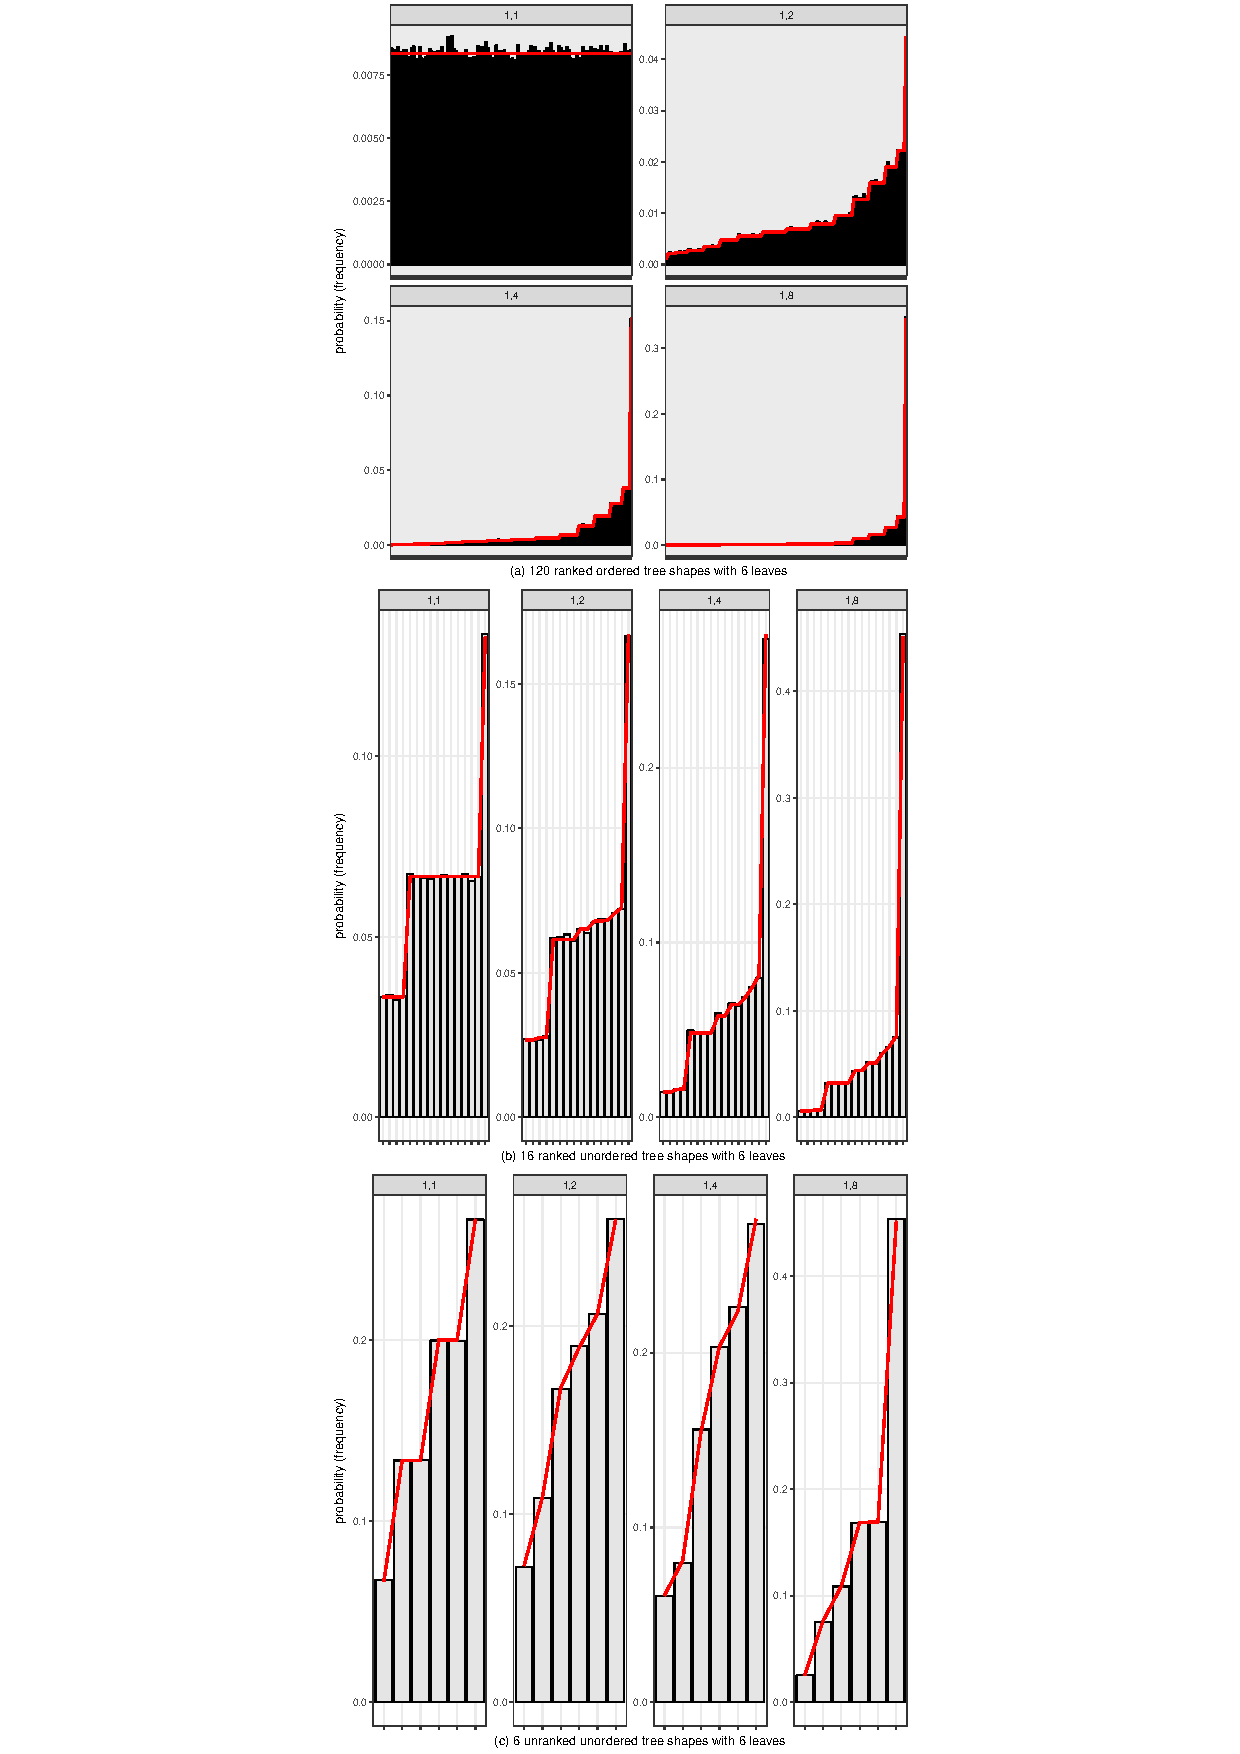
\includegraphics[width=0.35\textwidth]{figs/dualbirth-tree-prob-dists}
\caption[Probability distributions on ranked tree shapes]
{Probability distributions on ranked tree shapes. There are (a) 120 ranked ordered tree shapes, (b) 16 ranked unordered tree shapes, and (c) 6 unranked unordered tree shapes with $n=6$. The distribution according to the dual-birth model is given over these trees for four choices of $\la$ and $\lb$ (box header) corresponding to $r=1$ (i.e., Yule), $r=1/2$, $r=1/4$, and $r=1/8$. Red line gives the theoretical distribution and the grey bars give the frequencies in 100,000 simulations.}
\label{fig:dualbirth-tree-prob-dists}
\end{figure}

\begin{figure} % FIGURE S2 IN ORIGINAL PAPER
\centering
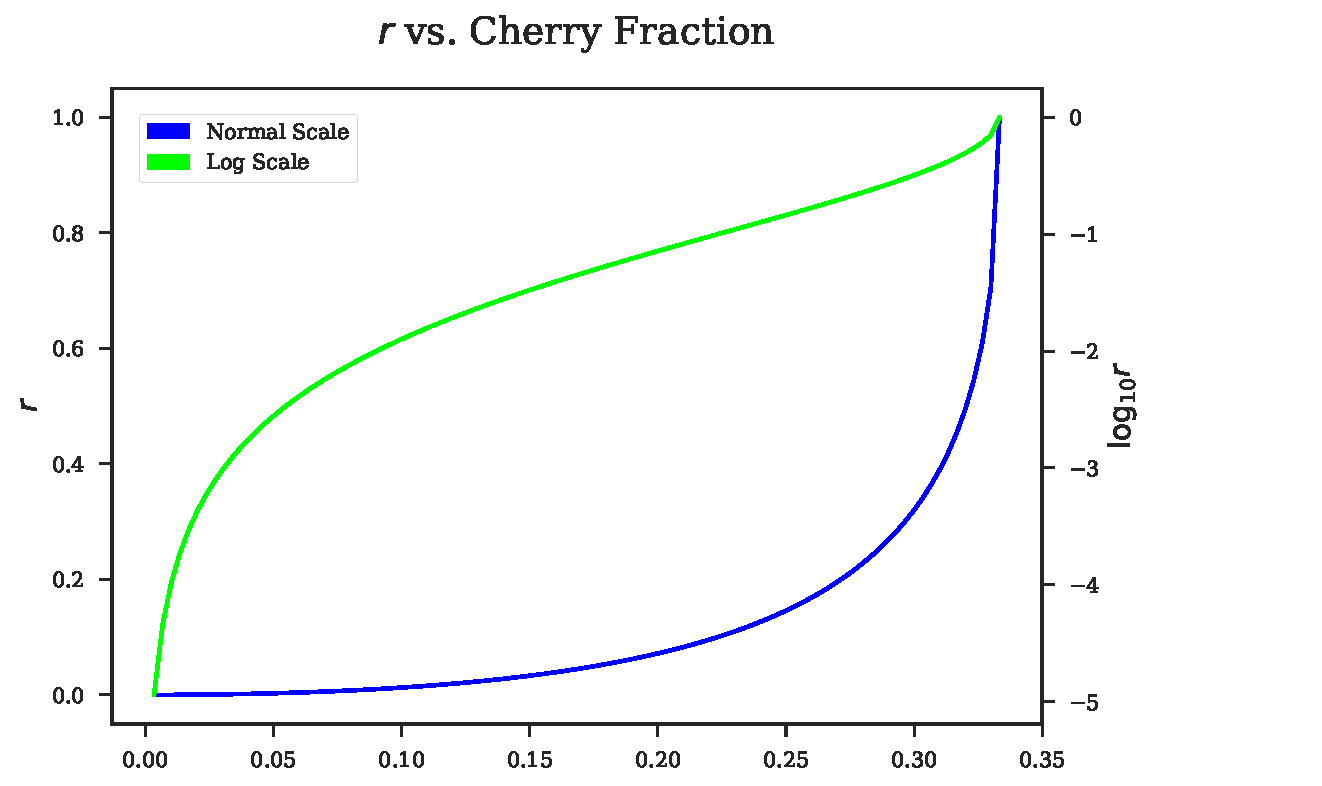
\includegraphics[width=0.8\textwidth]{figs/dualbirth-sup-cvsr}
\caption[Estimated $r$ vs. Cherry Fraction]
{Estimated $r$ vs. Cherry Fraction. Estimated $r$ (y-axis) as a function of the fraction of cherries (x-axis). Blue (left axis) shows normal scale and green (right) shows the logarithmic scale.}
\label{fig:dualbirth-sup-cvsr}
\end{figure}

\begin{figure} % FIGURE S3 IN ORIGINAL PAPER
\centering
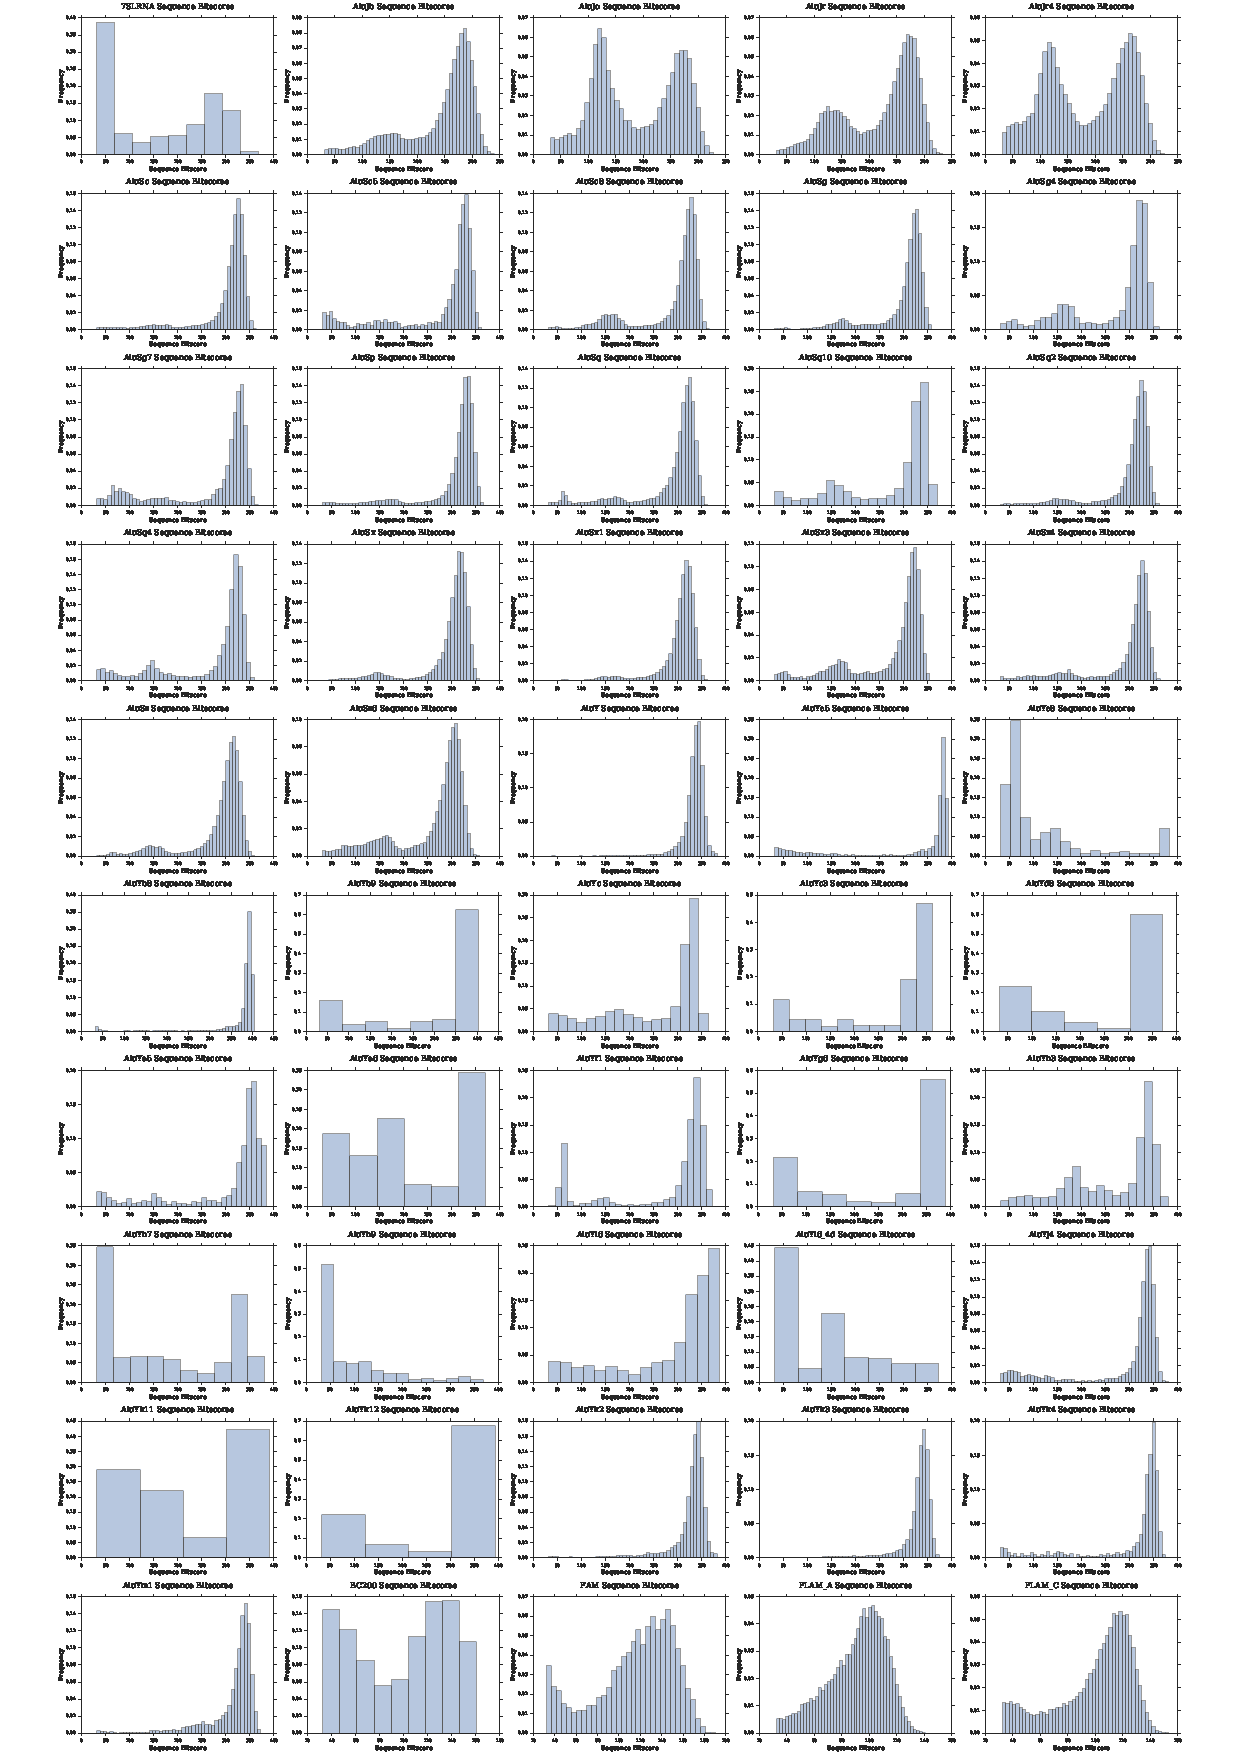
\includegraphics[width=0.8\textwidth]{figs/dualbirth-bit-hists}
\caption[Histograms of bitscores]
{Histograms of bitscores.}
\label{fig:dualbirth-bit-hists}
\end{figure}

\begin{figure} % FIGURE S4 IN ORIGINAL PAPER
\centering
\begin{small}
\begin{tabular}{c c c c c c c c}\hline
7SLRNA&AluJb&AluJo&AluJr&AluJr4&AluSc&AluSc5&AluSc8\\
200   &200  &200  &225  &200   &275  &275   &275\\\hline
AluSg&AluSg4&AluSg7&AluSp&AluSq&AluSq10&AluSq2&AluSq4\\
275  &275   &275   &275  &275  &275    &275   &250\\\hline
AluSx&AluSx1&AluSx3&AluSx4&AluSz&AluSz6&AluY&AluYa5\\
250  &250   &250   &250   &250  &250   &300 &325\\\hline
AluYa8&AluYb8&AluYb9&AluYc&AluYc3&AluYd8&AluYe5&AluYe6\\
100   &250   &250   &275  &300   &300   &300   &300\\\hline
AluYf1&AluYg6&AluYh3&AluYh7&AluYh9&AluYi6&AluYi6\_4d&AluYj4\\
300   &300   &300   &275   &200   &225   &225       &300\\\hline
AluYk11&AluYk12&AluYk2&AluYk3&AluYk4&AluYm1&BC200&FAM\\
325    &325    &250   &250   &375   &300   &100  &65\\\hline
FLAM\_A&FLAM\_C\\
80     &80\\
\hline
\end{tabular}
\end{small}
\caption[Bitscore thresholds]
{Bitscore thresholds.}
\label{fig:dualbirth-bit-thresh}
\end{figure}

\begin{figure} % FIGURE S5 IN ORIGINAL PAPER
\centering
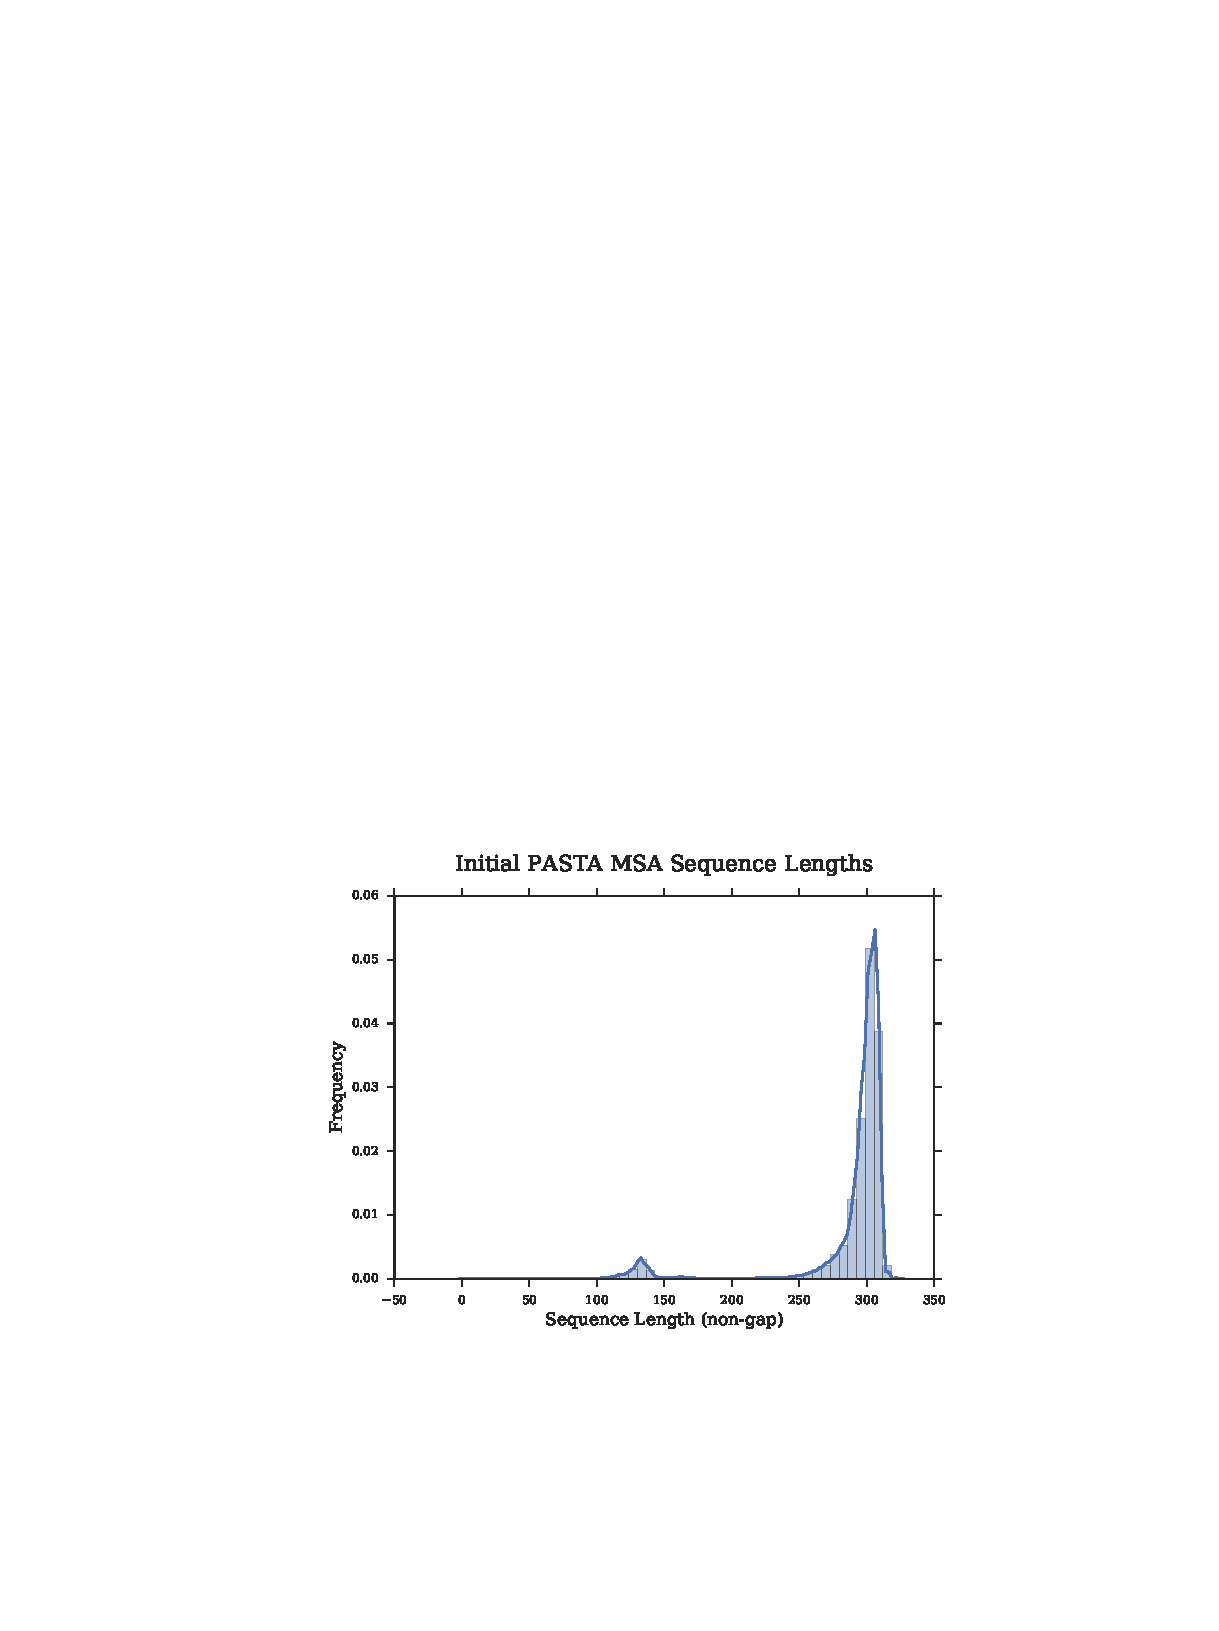
\includegraphics[width=0.9\textwidth]{figs/dualbirth-non-gap-hist}
\caption[PASTA alignment sequence lengths]
{PASTA alignment sequence lengths. Histogram of sequences based on non-gap sequence length. As can be seen, a nontrivial number of sequences in the alignment have non-gap lengths well below 300, which we know \textit{a priori} to be the typical length of \textit{ Alu} sequences.}
\label{fig:dualbirth-non-gap-hist}
\end{figure}

\begin{figure} % FIGURE S6 IN ORIGINAL PAPER
\begin{center}
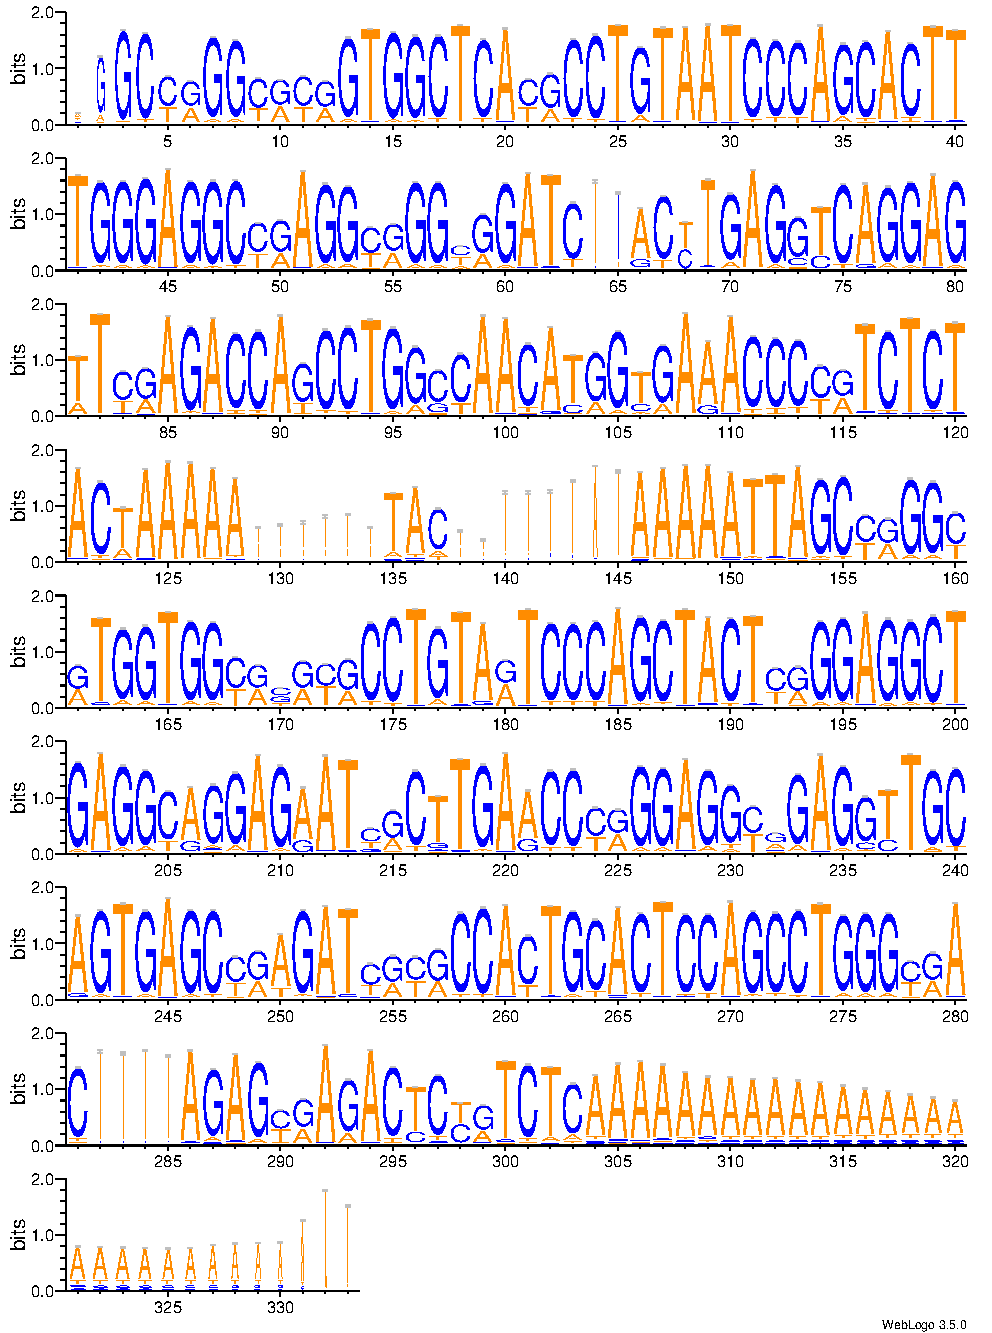
\includegraphics[width=0.45\textwidth]{figs/dualbirth-alu-tree-a.pdf}
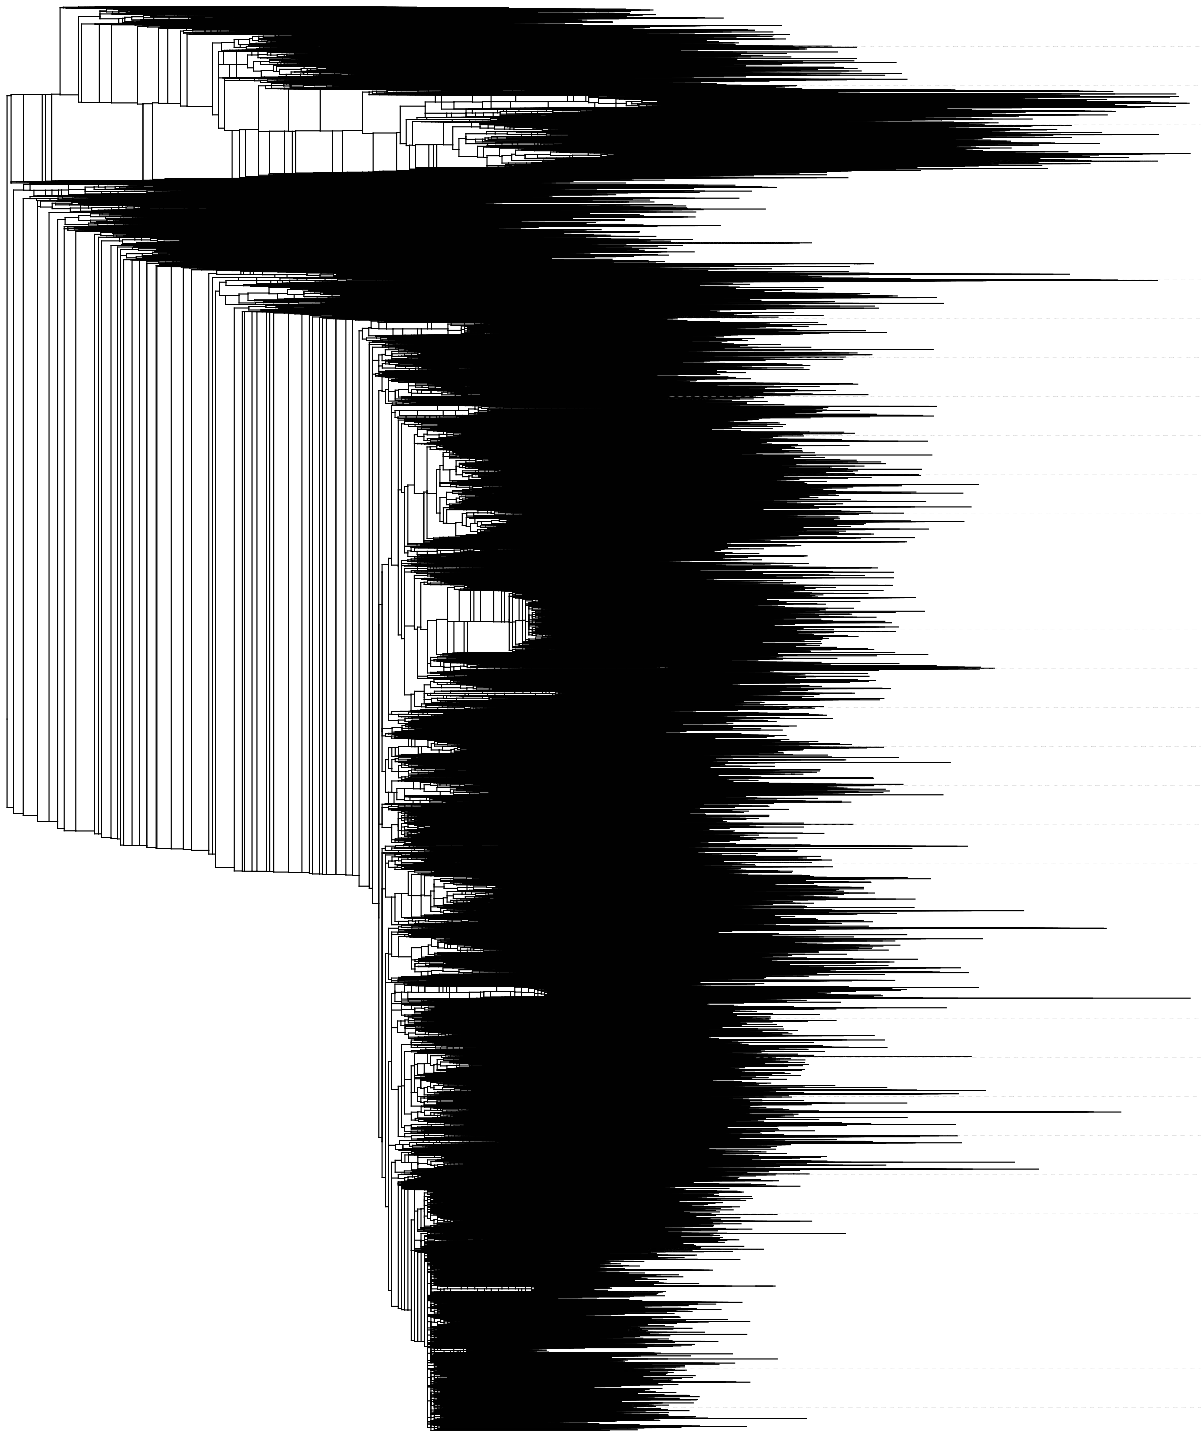
\includegraphics[width=0.45\textwidth]{figs/dualbirth-alu-tree-b.pdf}\\
(a)~~~~~~~~~~~~~~~~~~~~~~~~~~~~~~~~~~~~~~~~~~~~~~~~~~~~~~~~~~~~~~~~~(b)
\end{center}
\caption[Human \textit{Alu} alignment and tree]
{Human \textit{ Alu} alignment and tree. 
(a) Sequence logo constructed from the \textit{ Alu} multiple sequence alignment in which sequences with less than 200 non-gap characters were removed and sites with less than 1\% non-gap characters were masked, using WebLogo~\cite{Crooks2004}. The logo indicates conserved sequences and a good quality alignment: most sites have a clear high-frequency consensus nucleotide.\label{fig:dualbirth-alu-logo} (b) Midpoint-rooted \textit{ Alu} phylogenetic tree inferred from the aforementioned sequence alignment by RAxML under the \gls{GTR}+CAT model. As expected, portions of the tree are very ladder-like.}
\label{fig:dualbirth-alu-tree}
\end{figure}

\begin{figure} % FIGURE S7 IN ORIGINAL PAPER
\centering
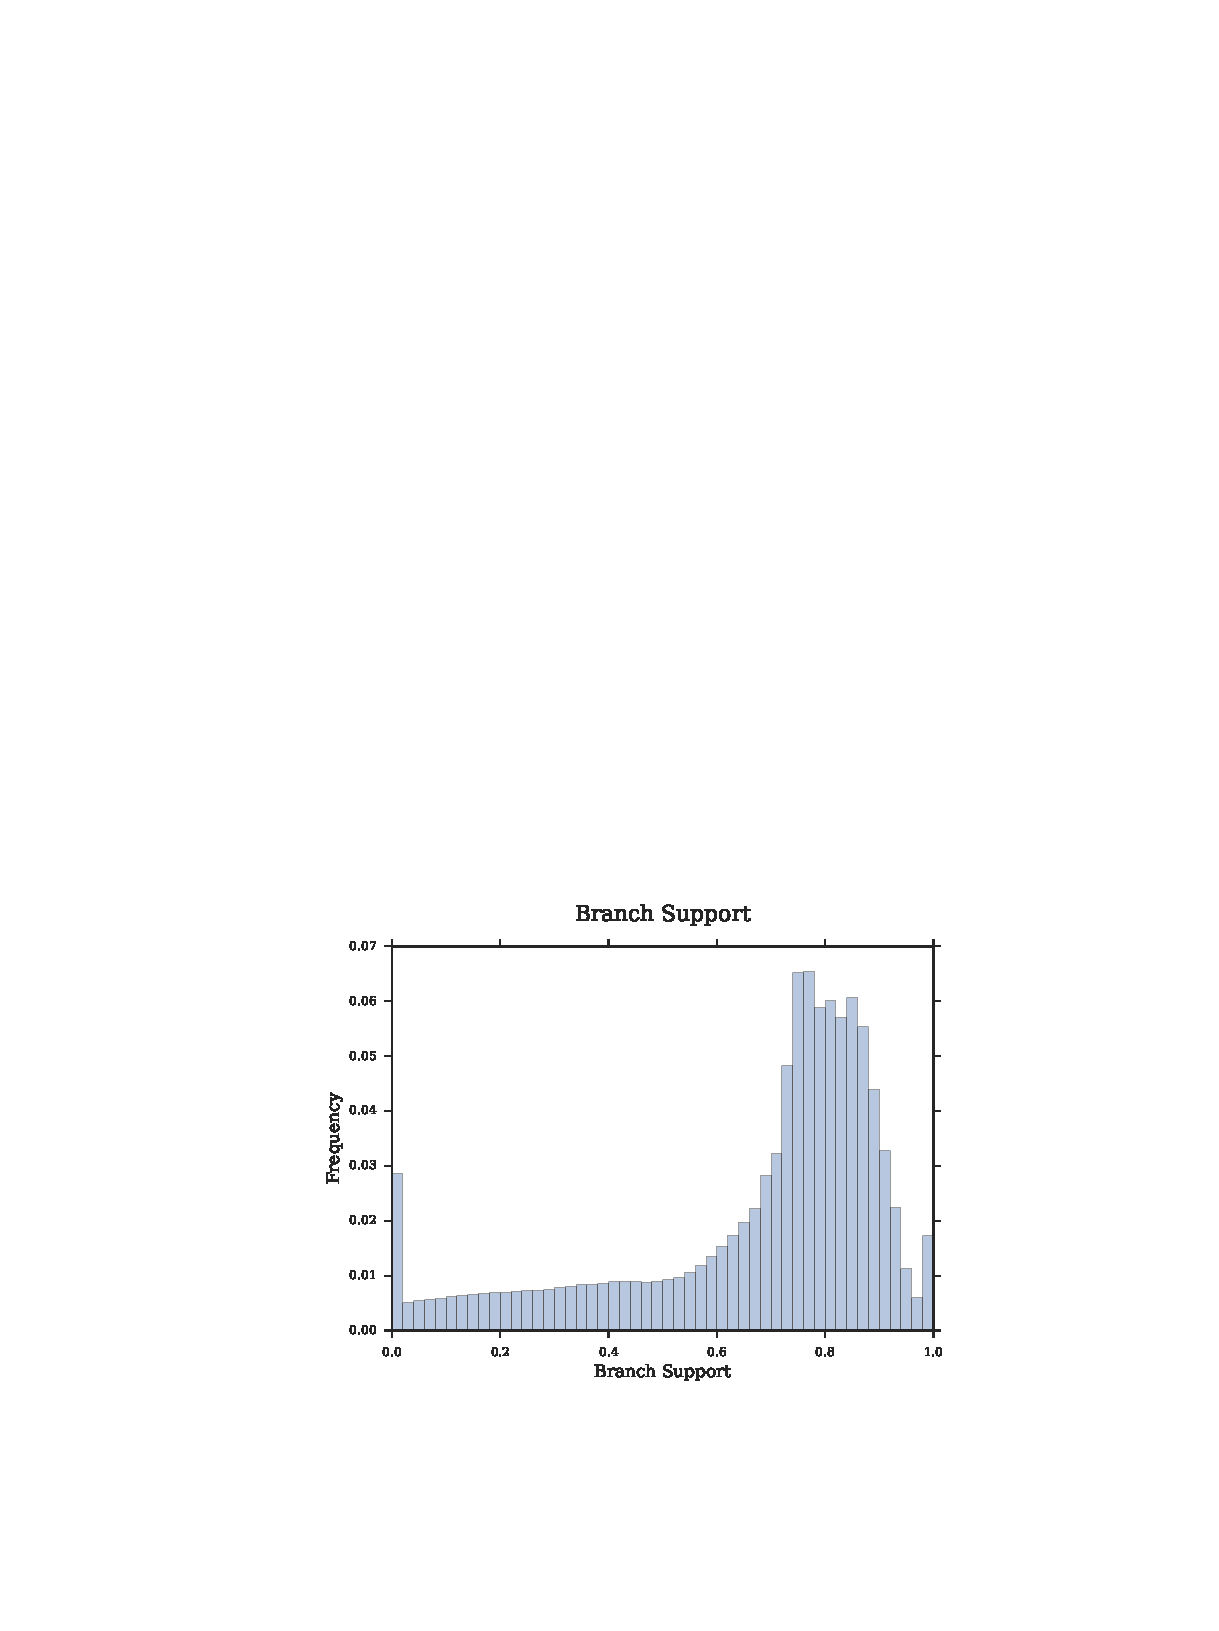
\includegraphics[width=0.8\textwidth]{figs/dualbirth-support-vals}
\caption[Human \textit{Alu} tree branch support]
{Human \textit{ Alu} tree branch support. Histogram of SH-like branch support values in the tree constructed from the masked alignment using FastTree~2. As can be seen, there are many low-support branches. Values below 0.9 are typically considered low SH-like support.}
\label{fig:dualbirth-support-vals}
\end{figure}

\begin{figure} % FIGURE S8 IN ORIGINAL PAPER
\centering
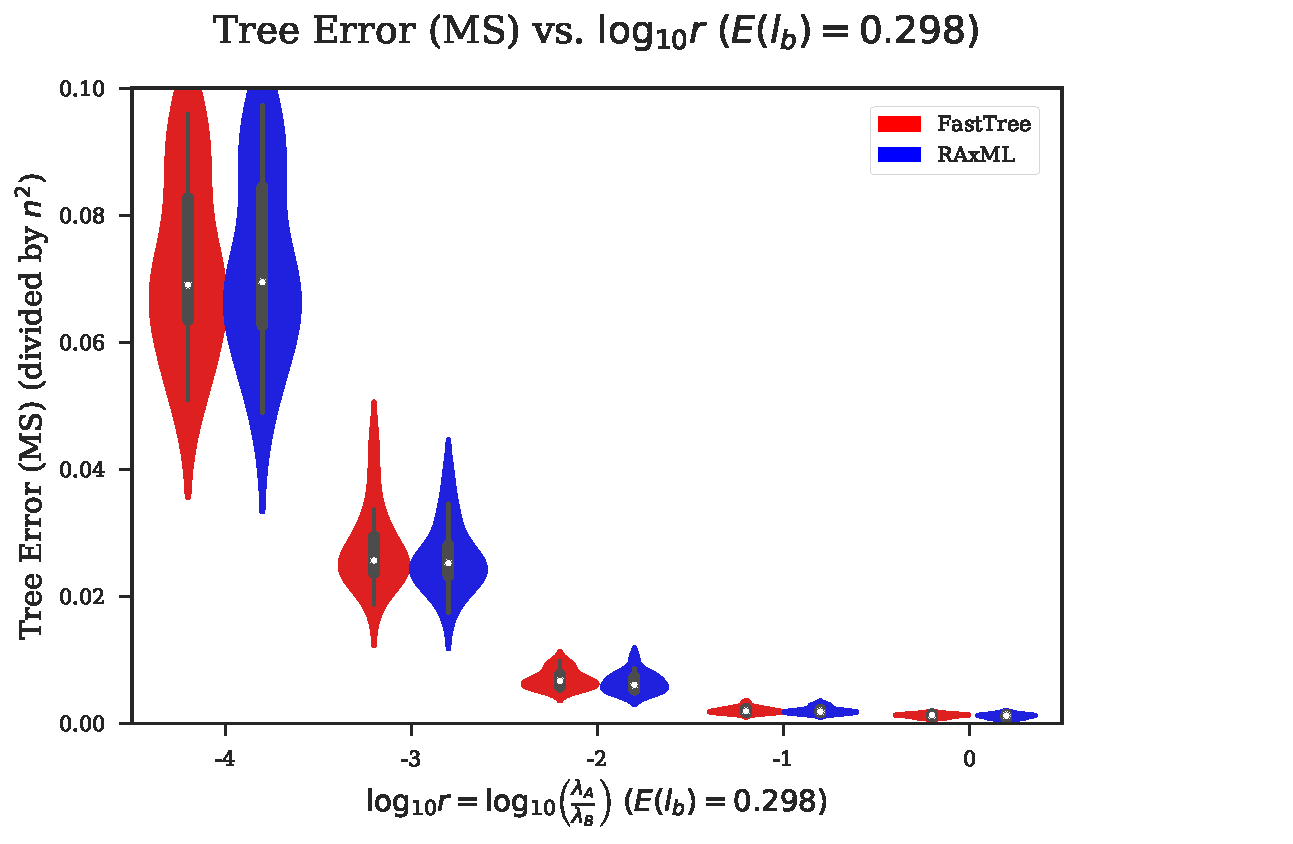
\includegraphics[width=0.3\textwidth]{figs/dualbirth-tree-ms-a}
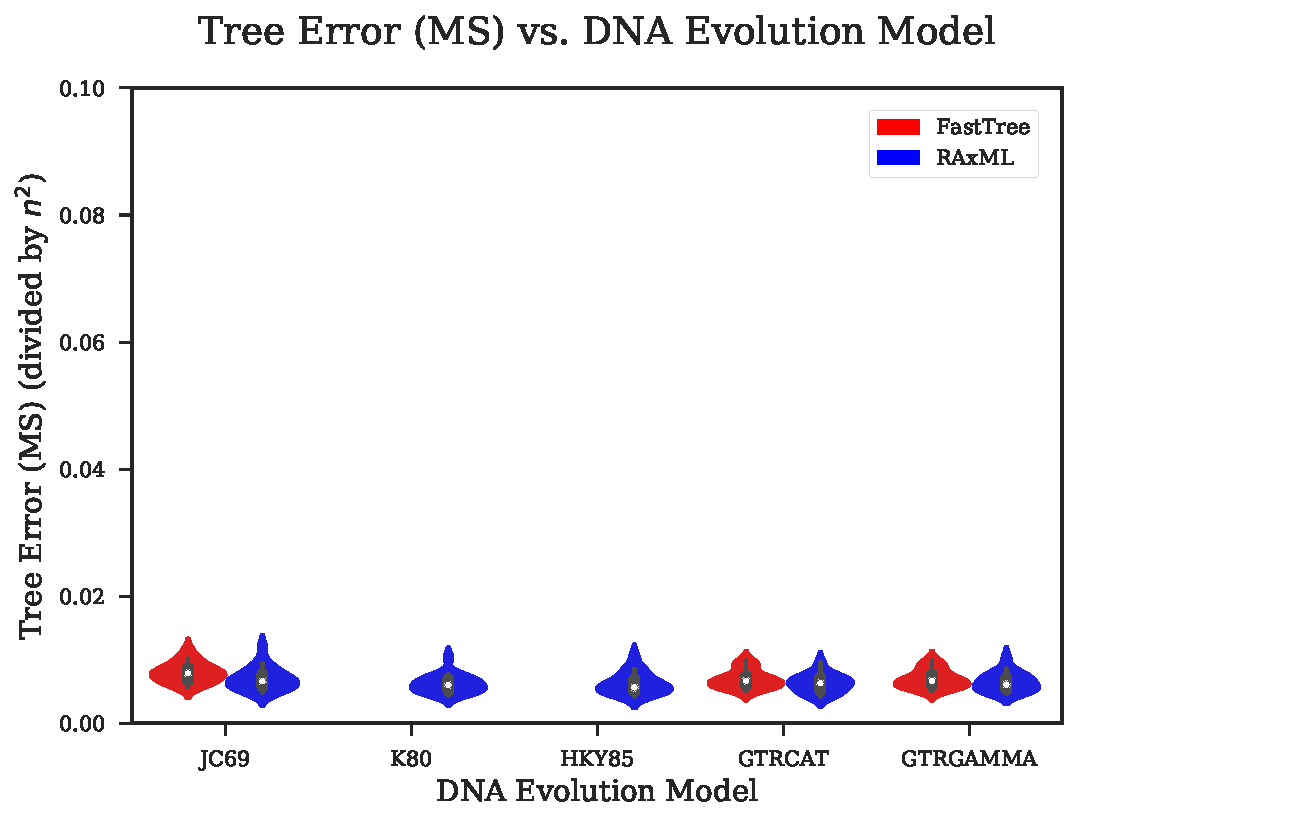
\includegraphics[width=0.3\textwidth]{figs/dualbirth-tree-ms-b}
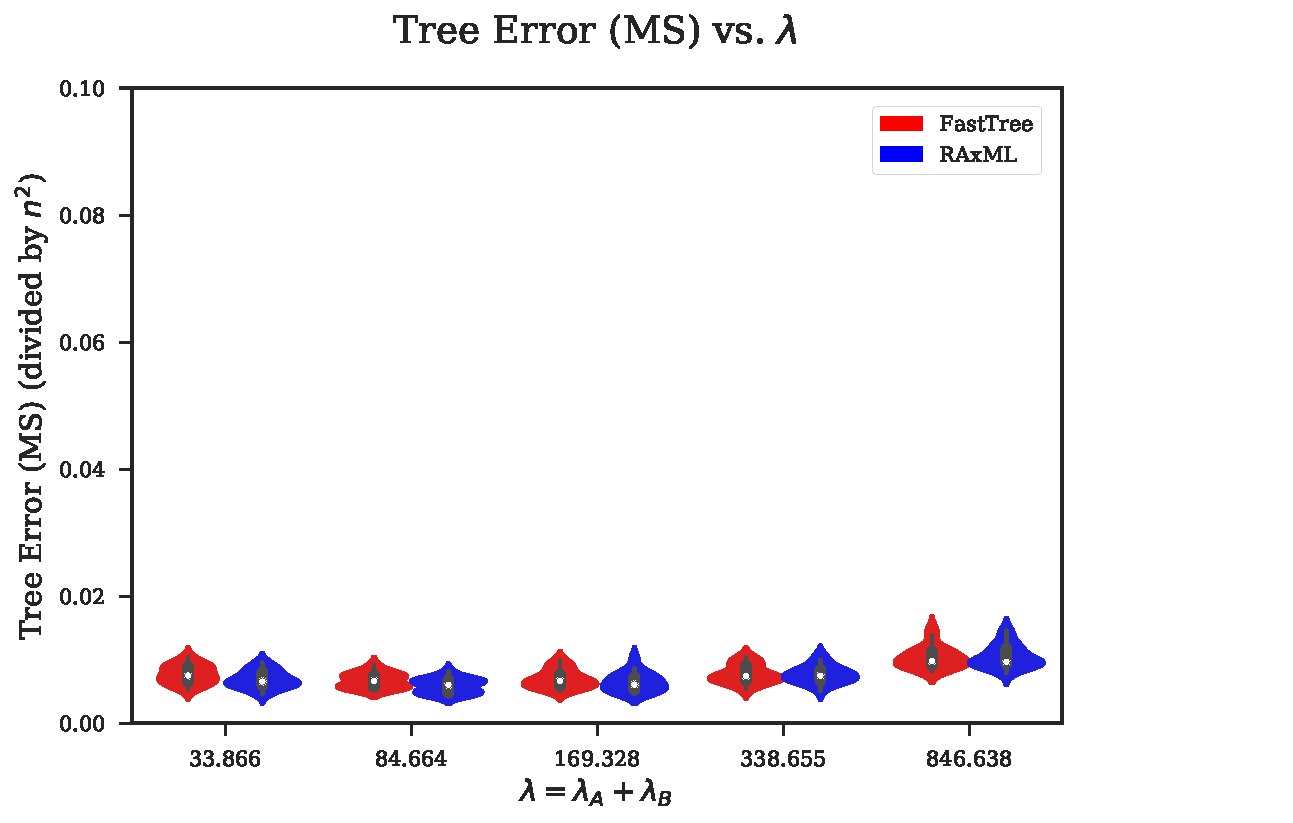
\includegraphics[width=0.3\textwidth]{figs/dualbirth-tree-ms-c}\\
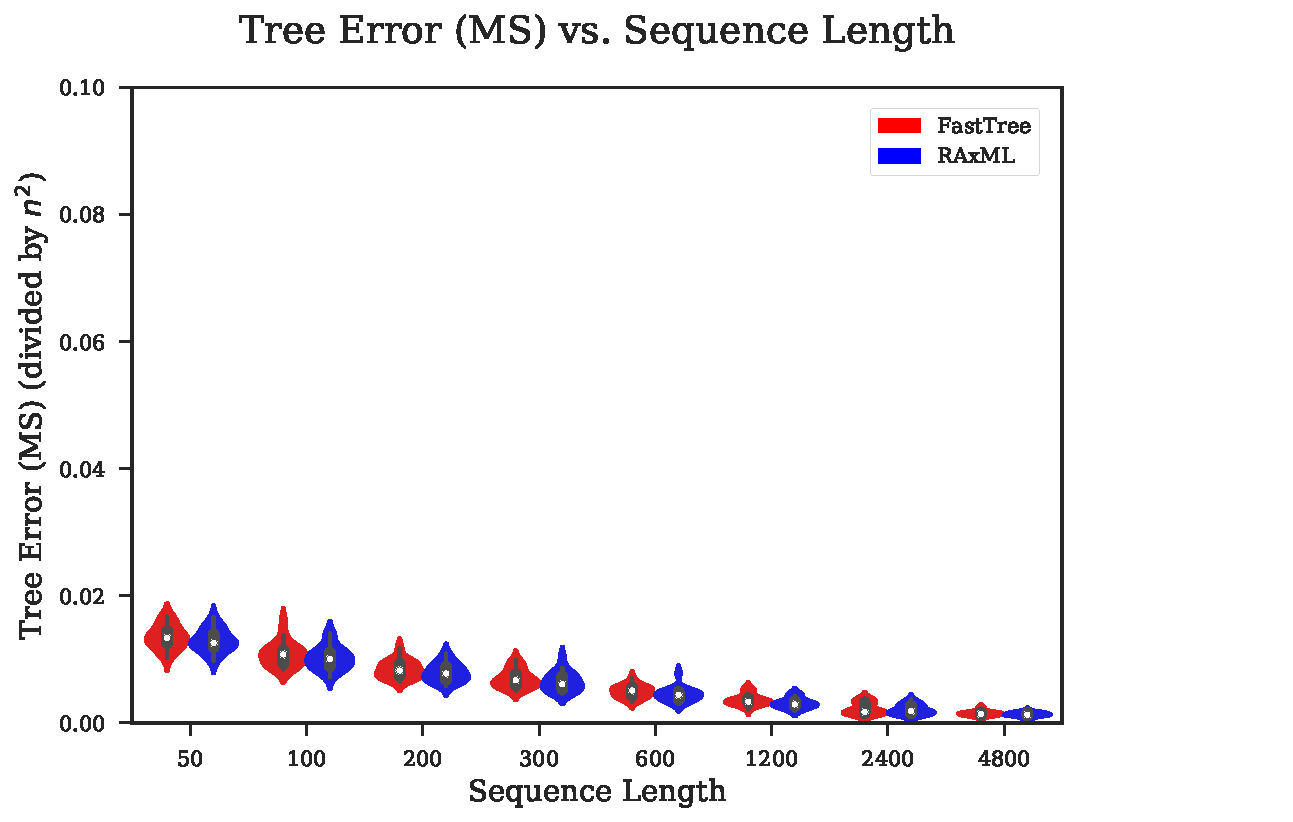
\includegraphics[width=0.3\textwidth]{figs/dualbirth-tree-ms-d}
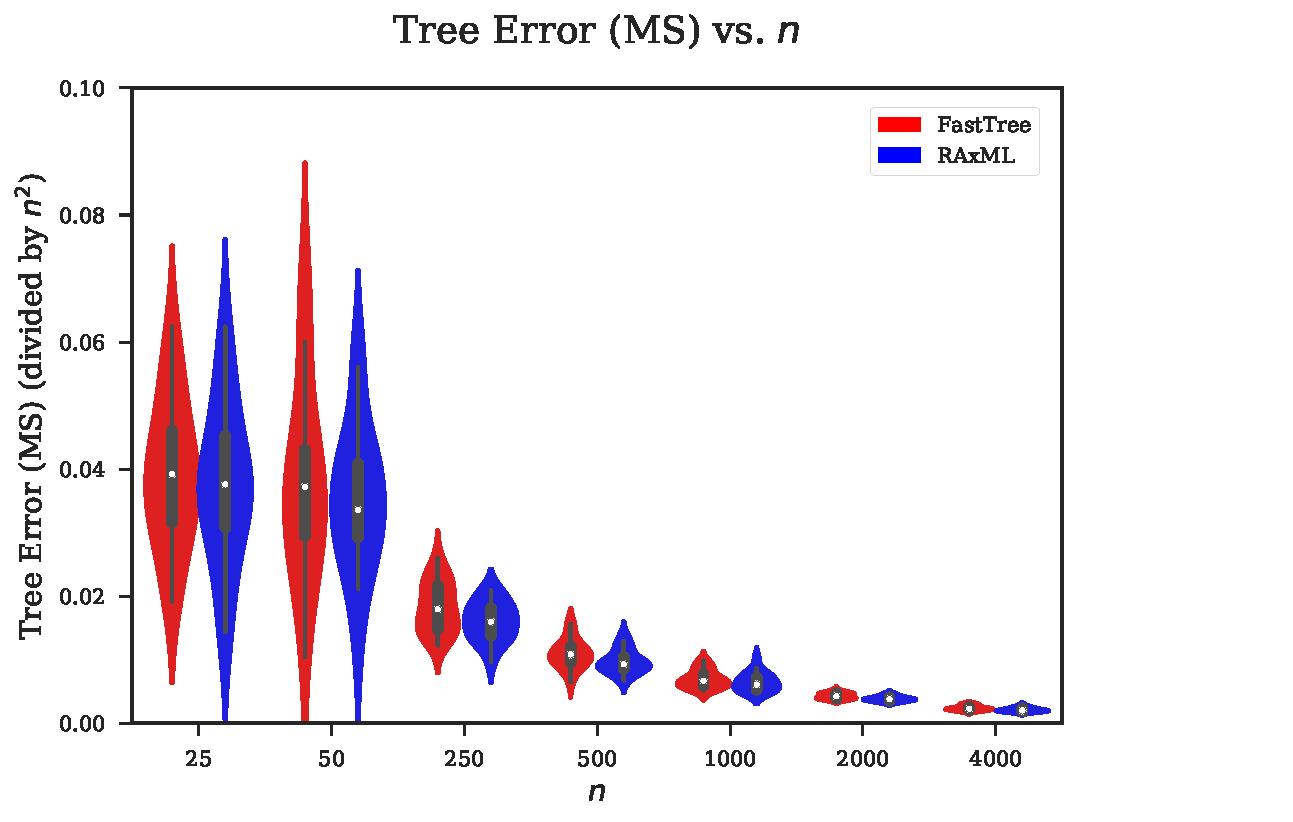
\includegraphics[width=0.3\textwidth]{figs/dualbirth-tree-ms-e}
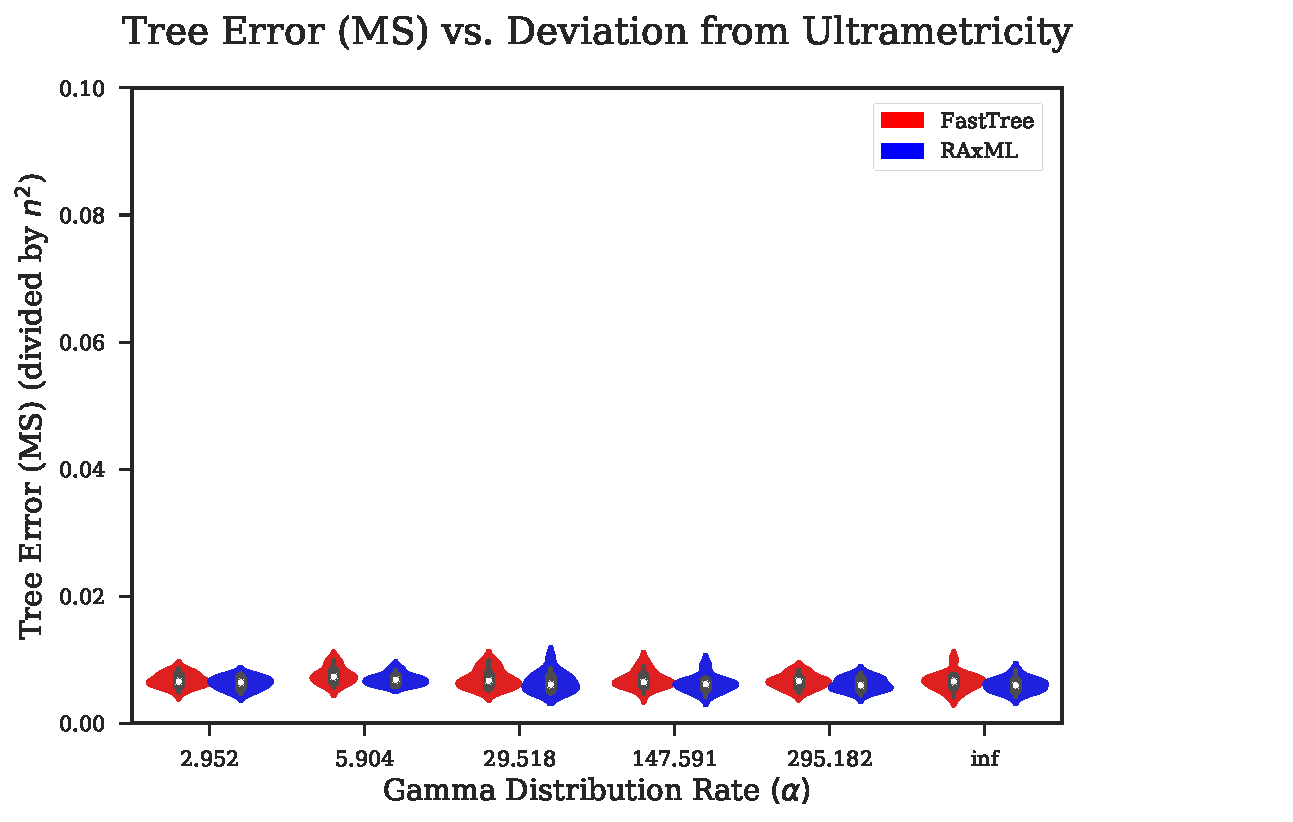
\includegraphics[width=0.3\textwidth]{figs/dualbirth-tree-ms-f}
\caption[Tree inference error (MS)]
{Tree inference error (MS). Violin plots are shown for the MS distance between true and estimated trees.}
\label{fig:dualbirth-tree-ms}
\end{figure}

\begin{figure} % FIGURE S9 IN ORIGINAL PAPER
\centering
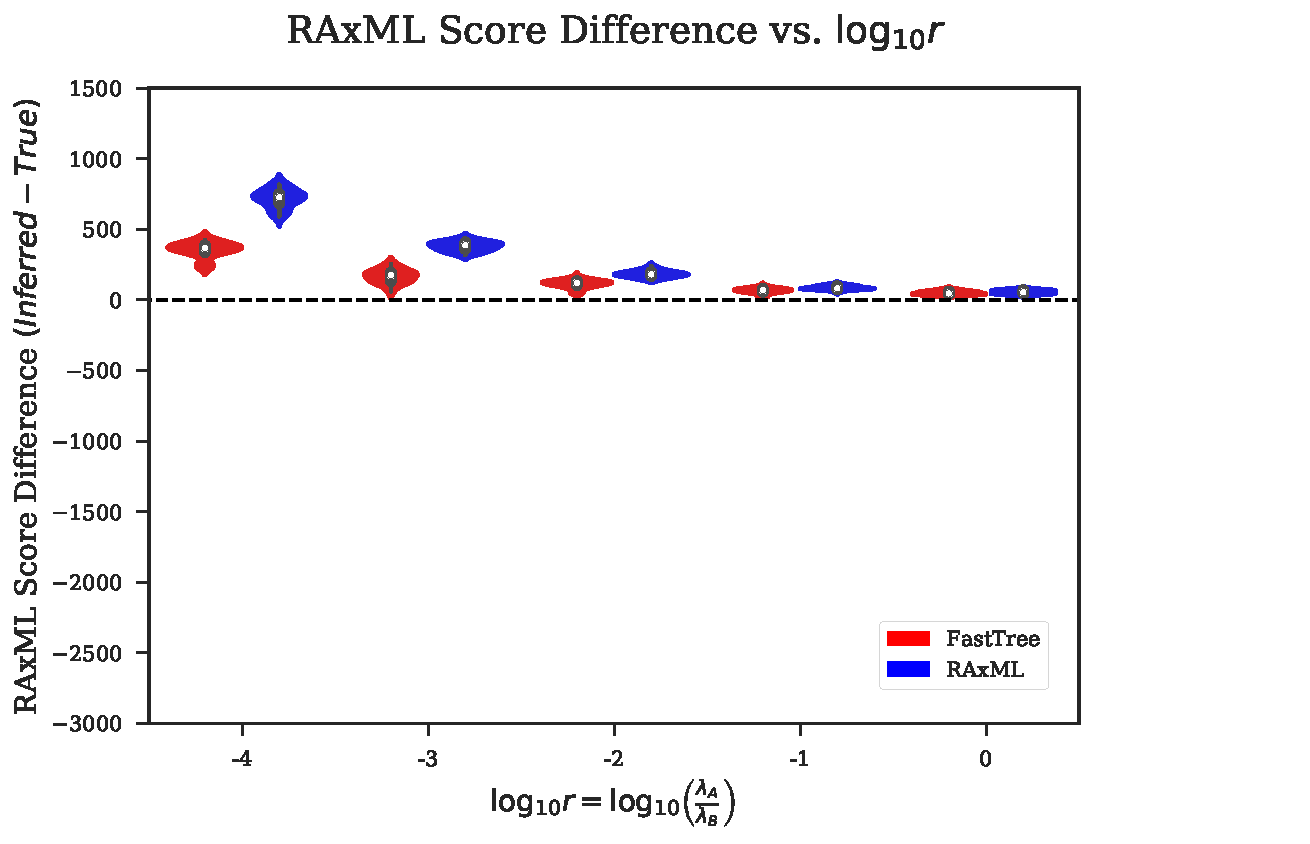
\includegraphics[width=0.3\textwidth]{figs/dualbirth-tree-score-diff-a}
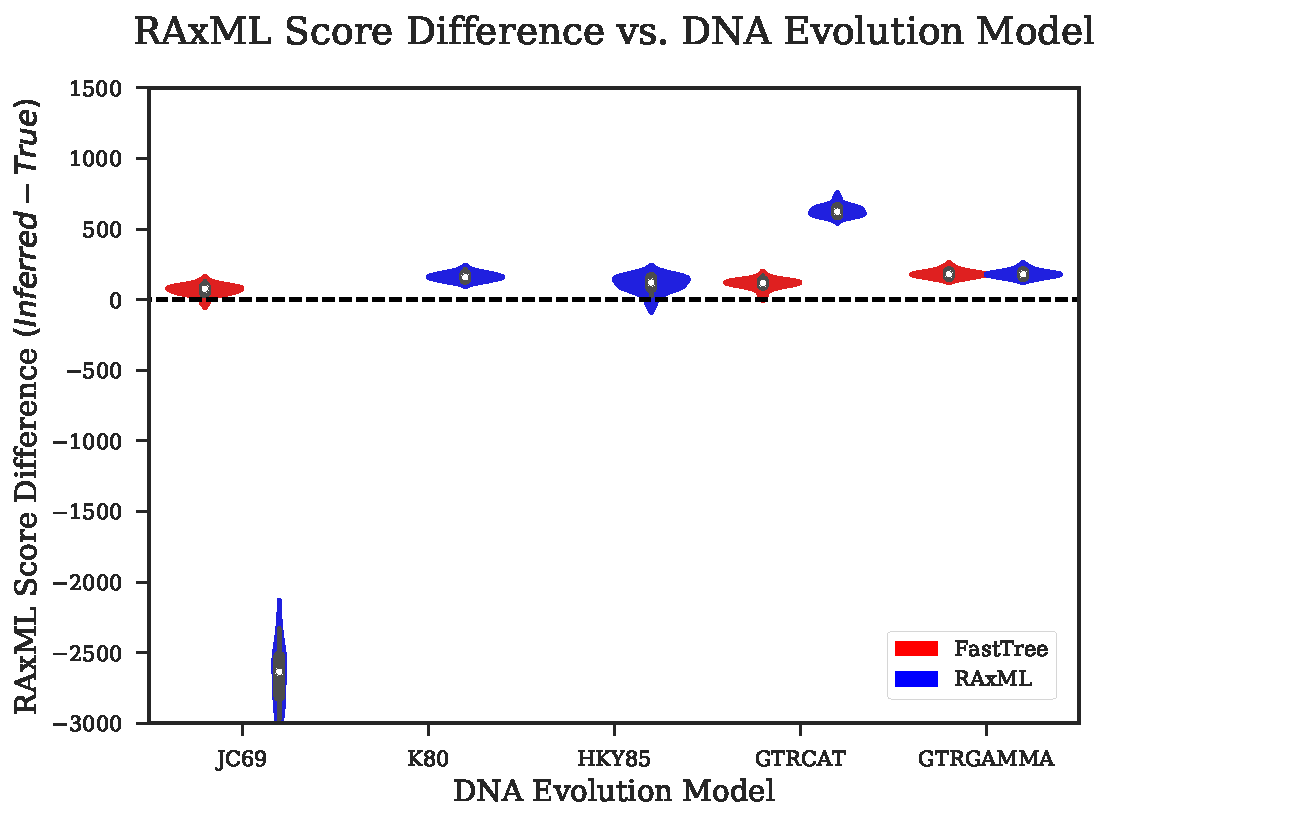
\includegraphics[width=0.3\textwidth]{figs/dualbirth-tree-score-diff-b}
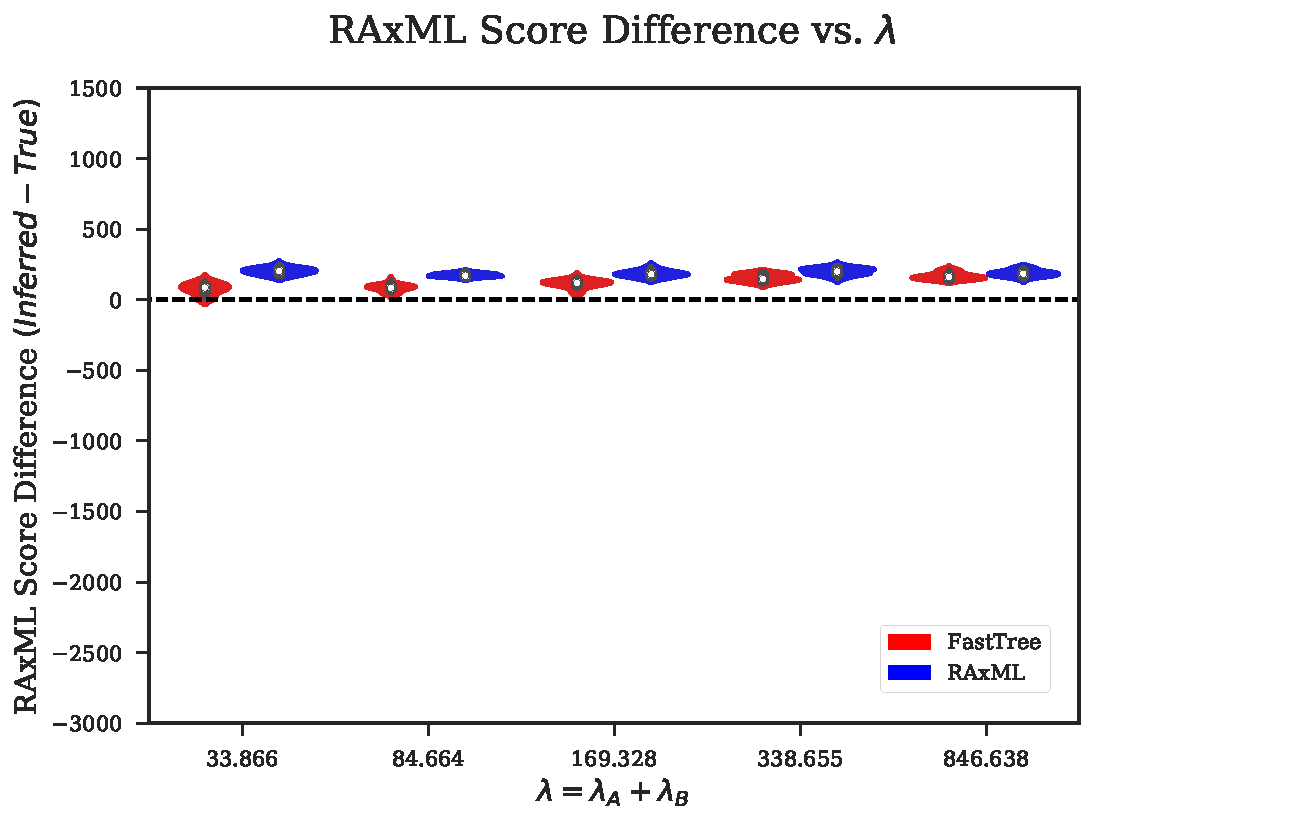
\includegraphics[width=0.3\textwidth]{figs/dualbirth-tree-score-diff-c}\\
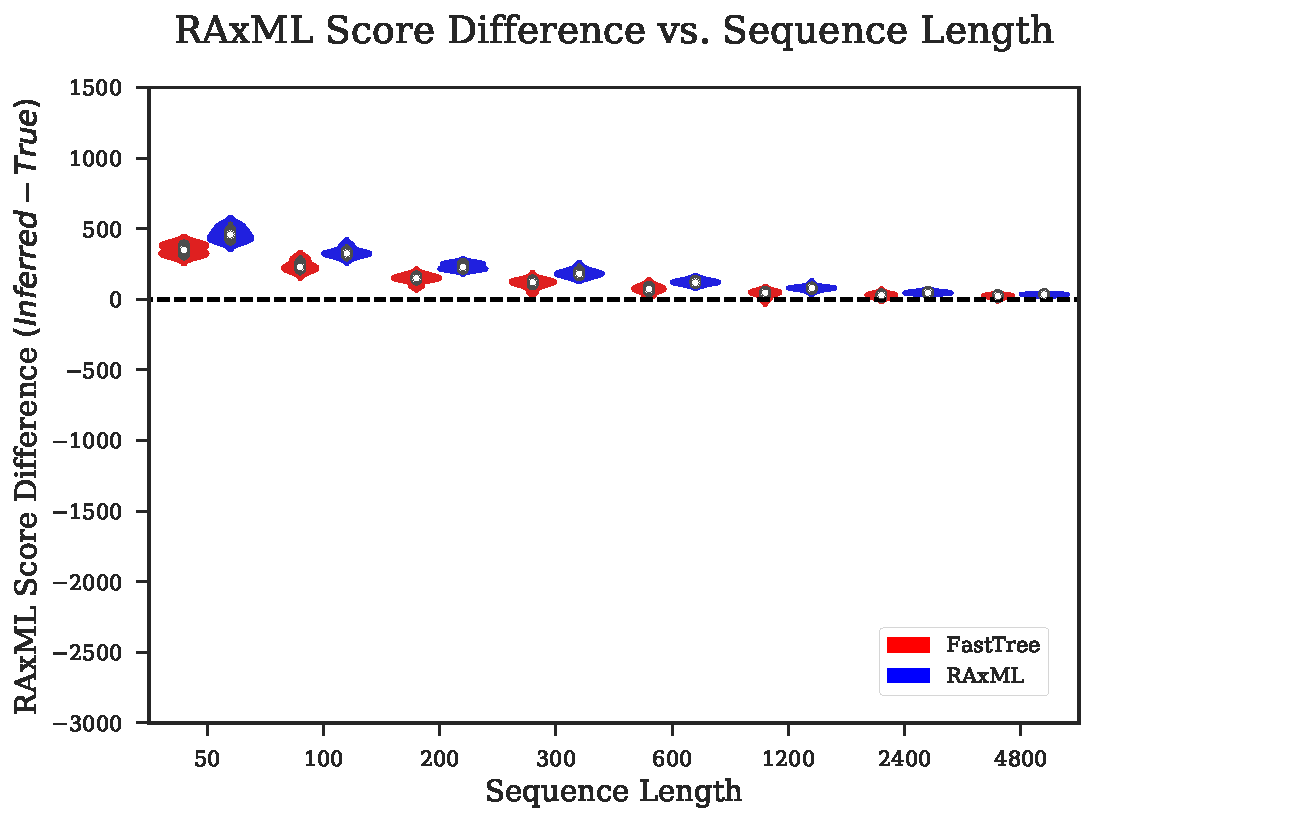
\includegraphics[width=0.3\textwidth]{figs/dualbirth-tree-score-diff-d}
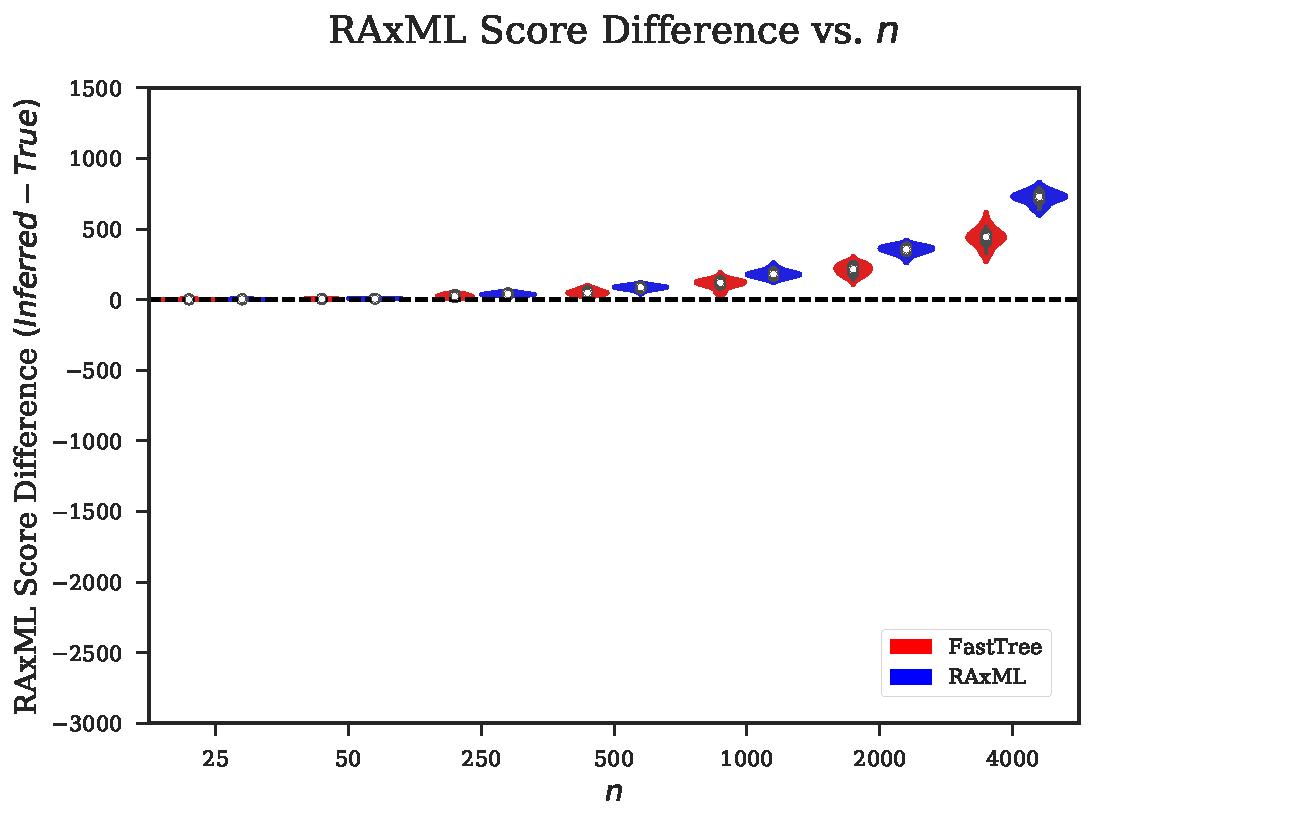
\includegraphics[width=0.3\textwidth]{figs/dualbirth-tree-score-diff-e}
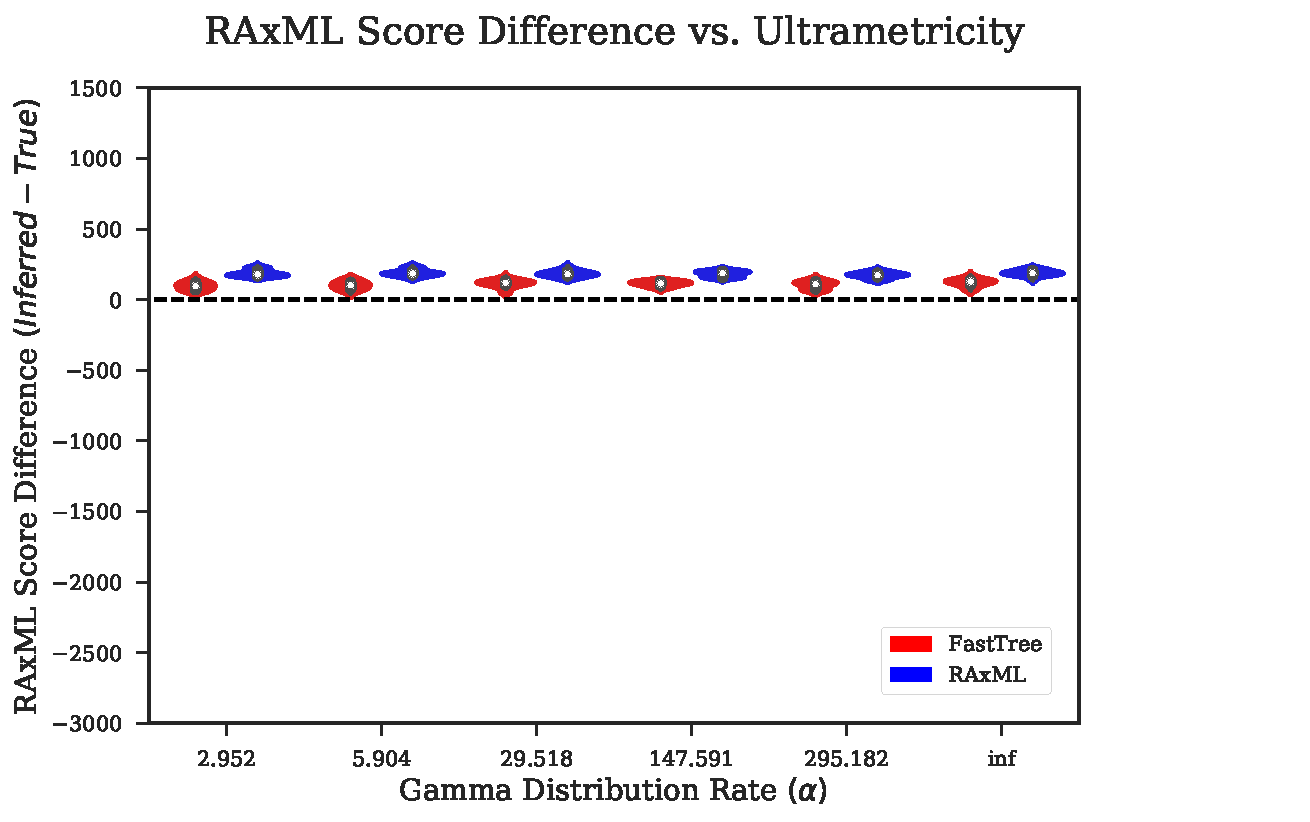
\includegraphics[width=0.3\textwidth]{figs/dualbirth-tree-score-diff-f}
\caption[Tree inference error]
{Tree inference error. Violin plots are shown for the log-likelihood score, as computed by RAxML, of the inferred tree minus the true tree; values away from zero indicate that the true tree has low log-likelihood scores.}
\label{fig:dualbirth-tree-score-diff}
\end{figure}

\begin{figure} % FIGURE S10 IN ORIGINAL PAPER
\centering
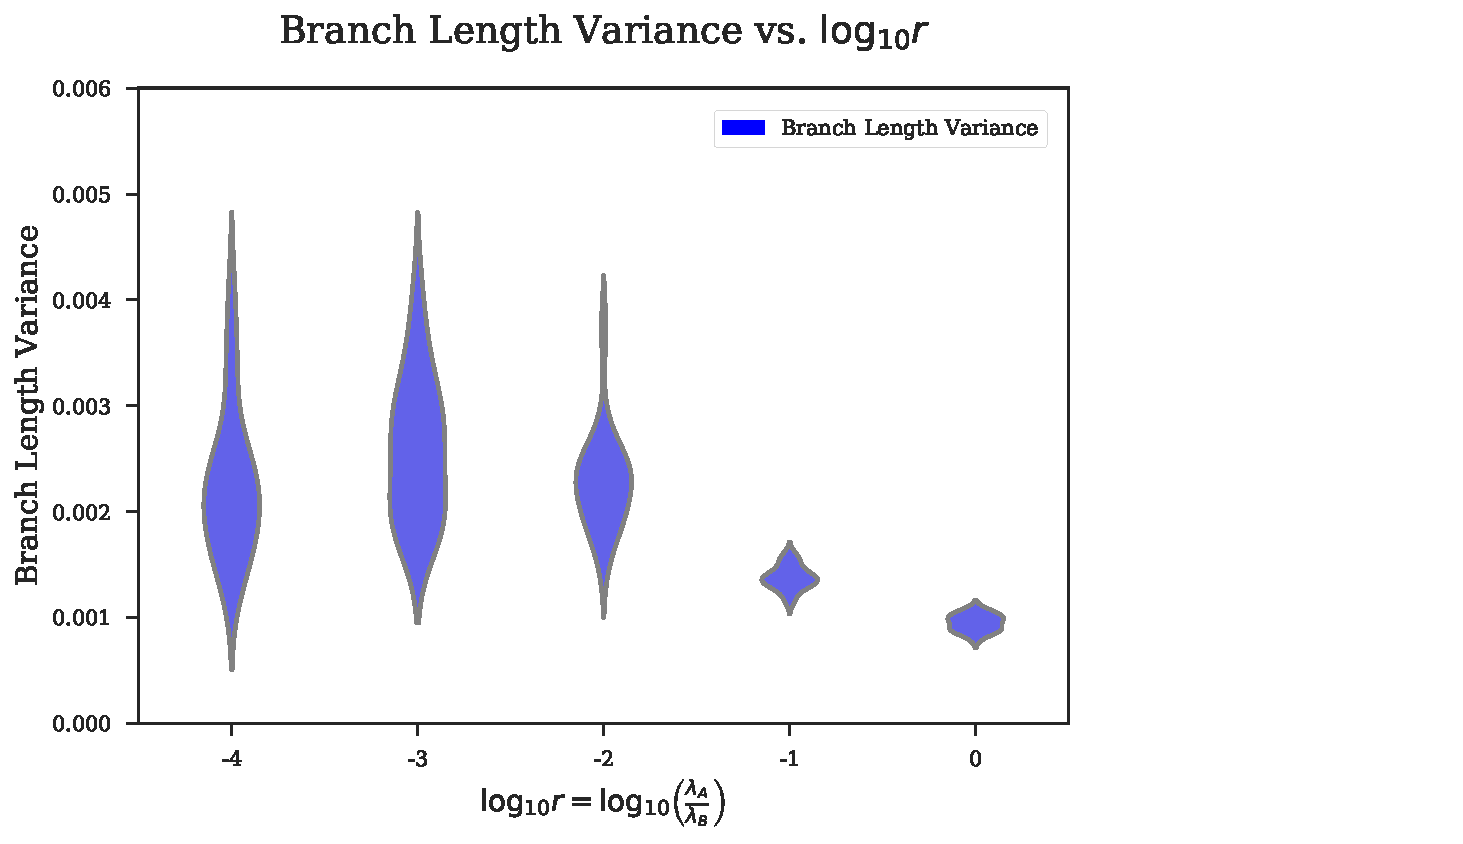
\includegraphics[width=0.3\textwidth]{figs/dualbirth-tree-bl-supp-a}
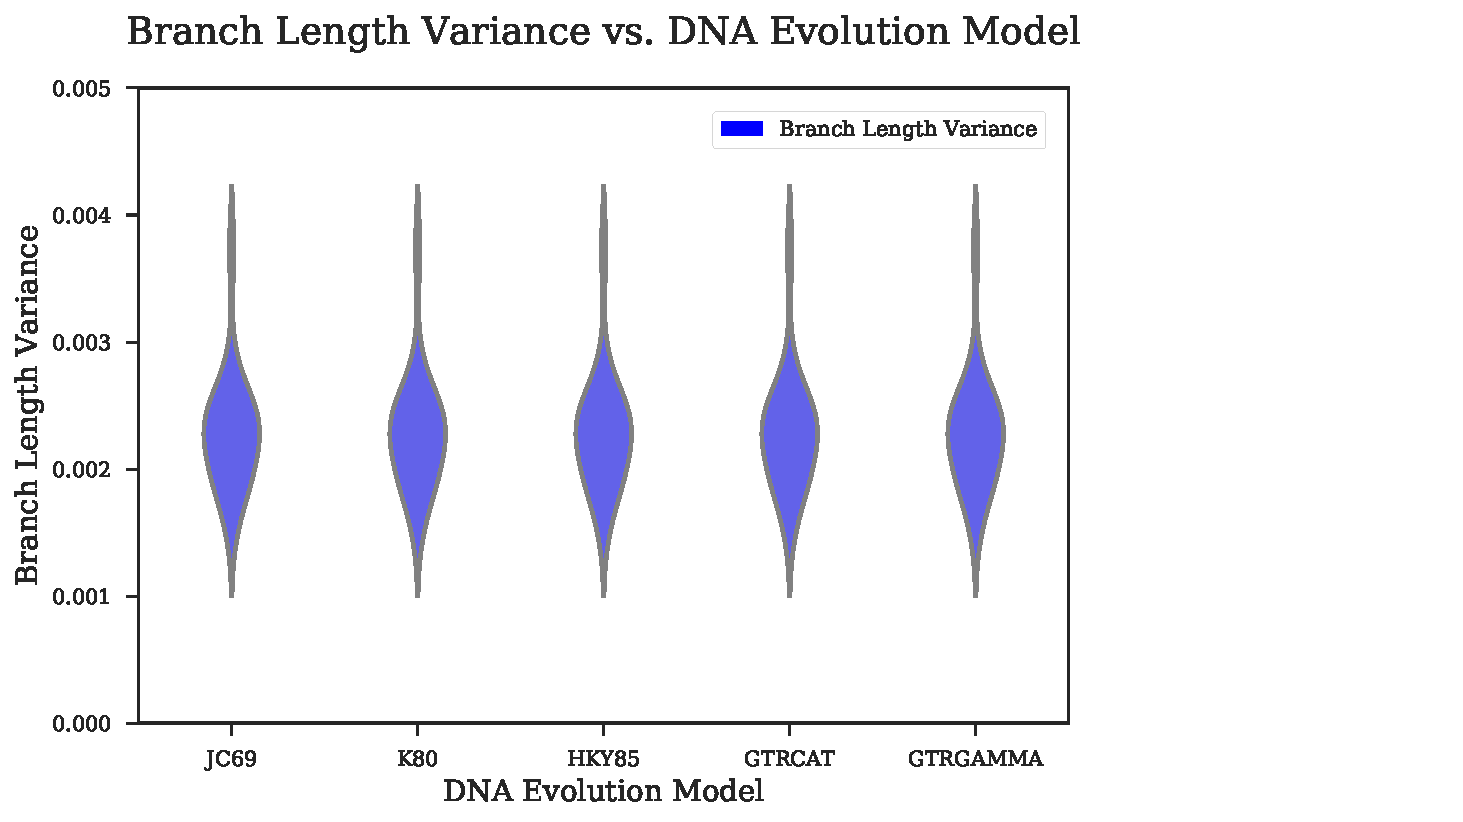
\includegraphics[width=0.3\textwidth]{figs/dualbirth-tree-bl-supp-b}
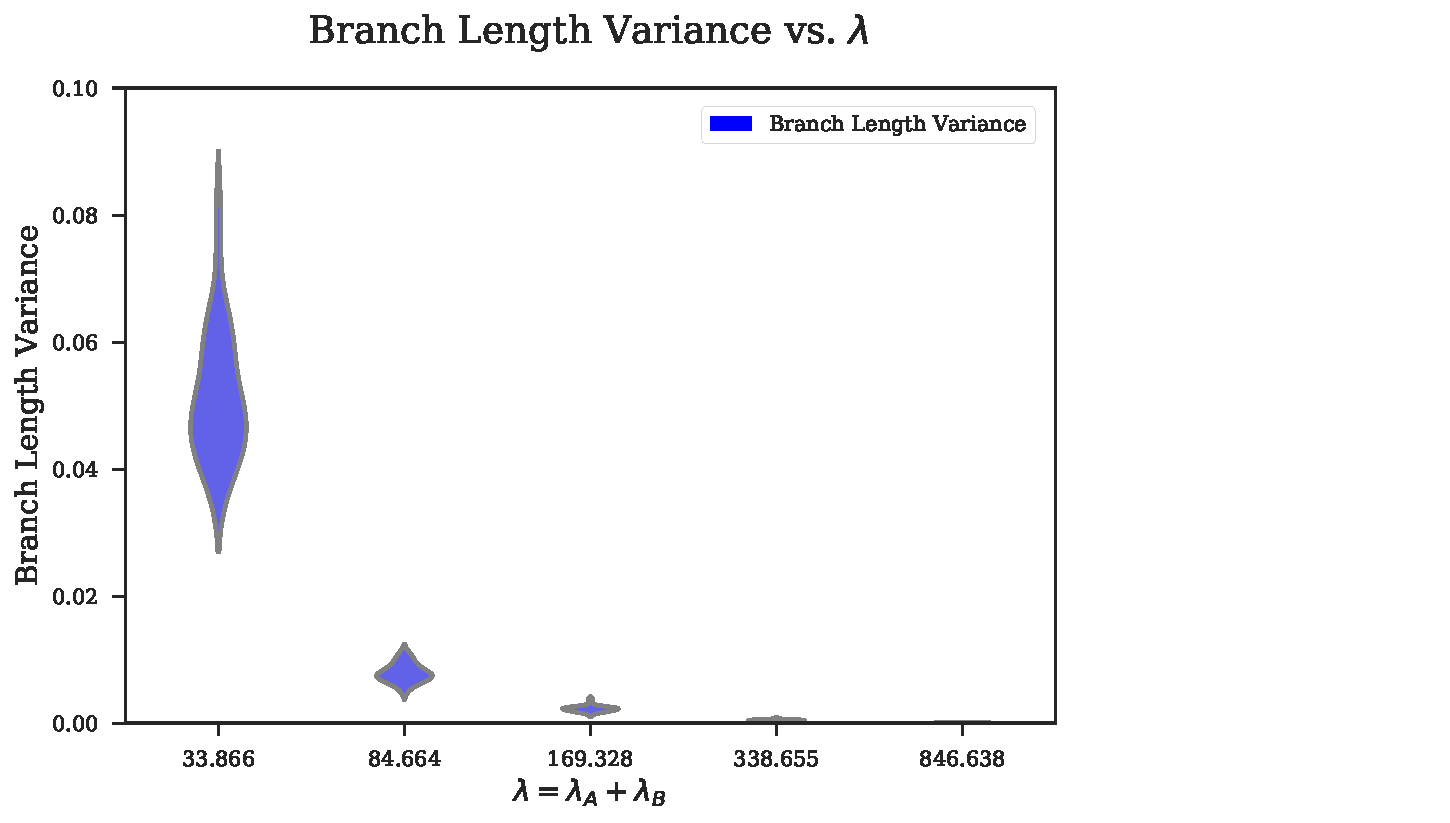
\includegraphics[width=0.3\textwidth]{figs/dualbirth-tree-bl-supp-c}\\
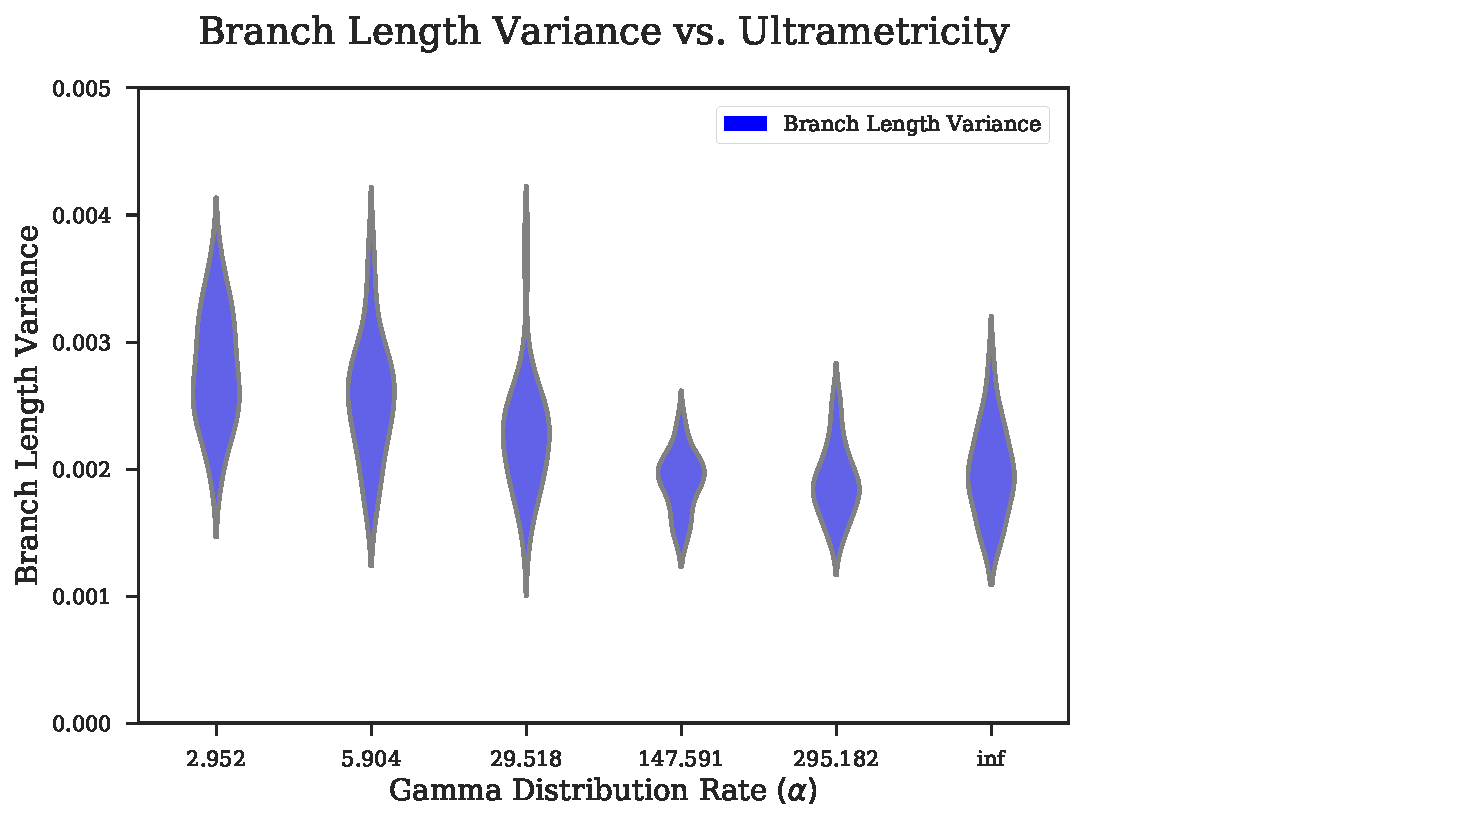
\includegraphics[width=0.3\textwidth]{figs/dualbirth-tree-bl-supp-d}
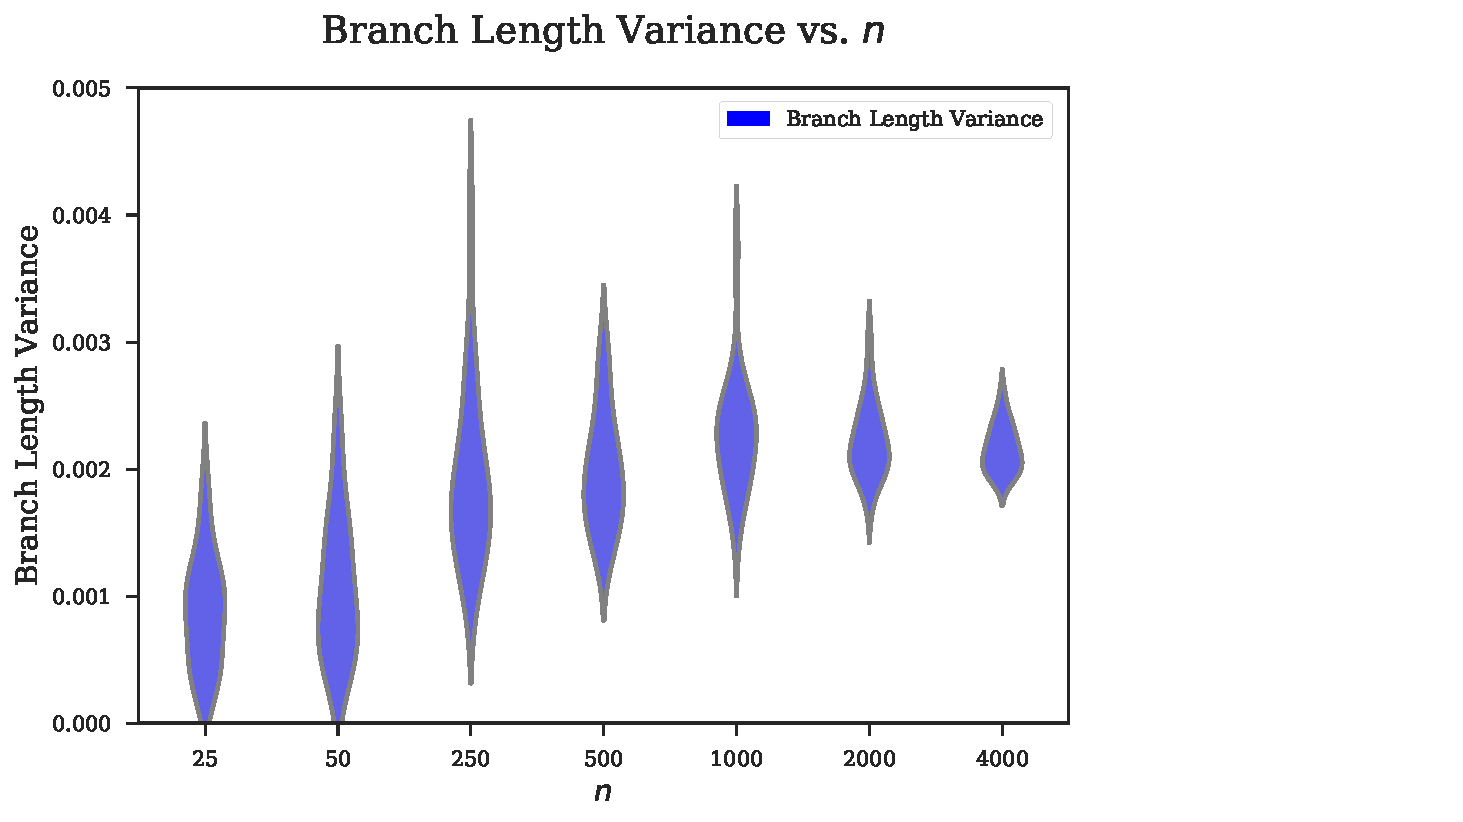
\includegraphics[width=0.3\textwidth]{figs/dualbirth-tree-bl-supp-e}
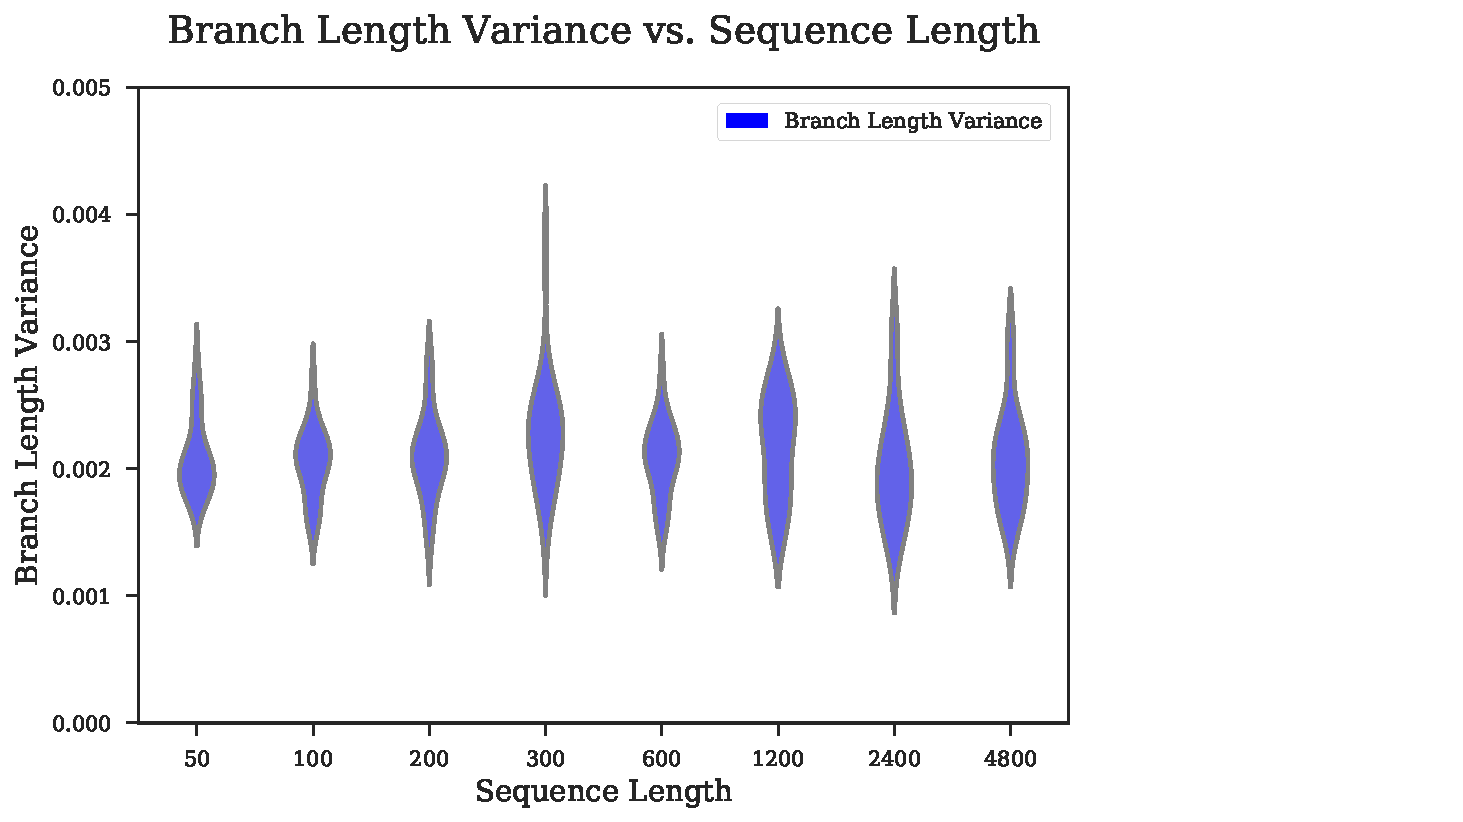
\includegraphics[width=0.3\textwidth]{figs/dualbirth-tree-bl-supp-f}
\caption[Branch length summary statistics]
{Branch length summary statistics. Violin plots are shown for the branch length variance computed for true trees.}
\label{fig:dualbirth-tree-bl-supp}
\end{figure}

\begin{figure} % FIGURE S11 IN ORIGINAL PAPER
\centering
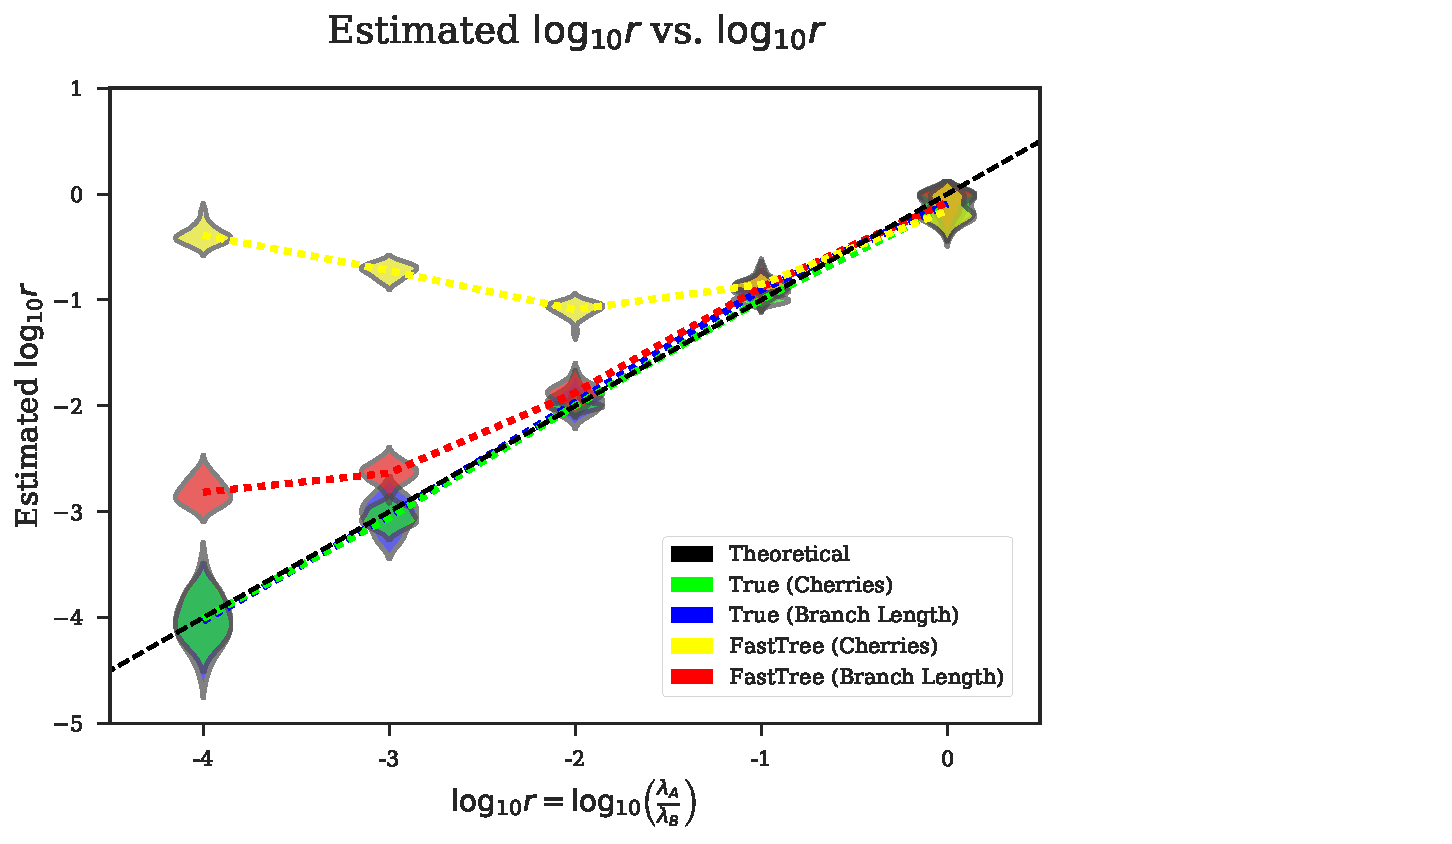
\includegraphics[width=0.3\textwidth]{figs/dualbirth-res-cherry-supp-a}
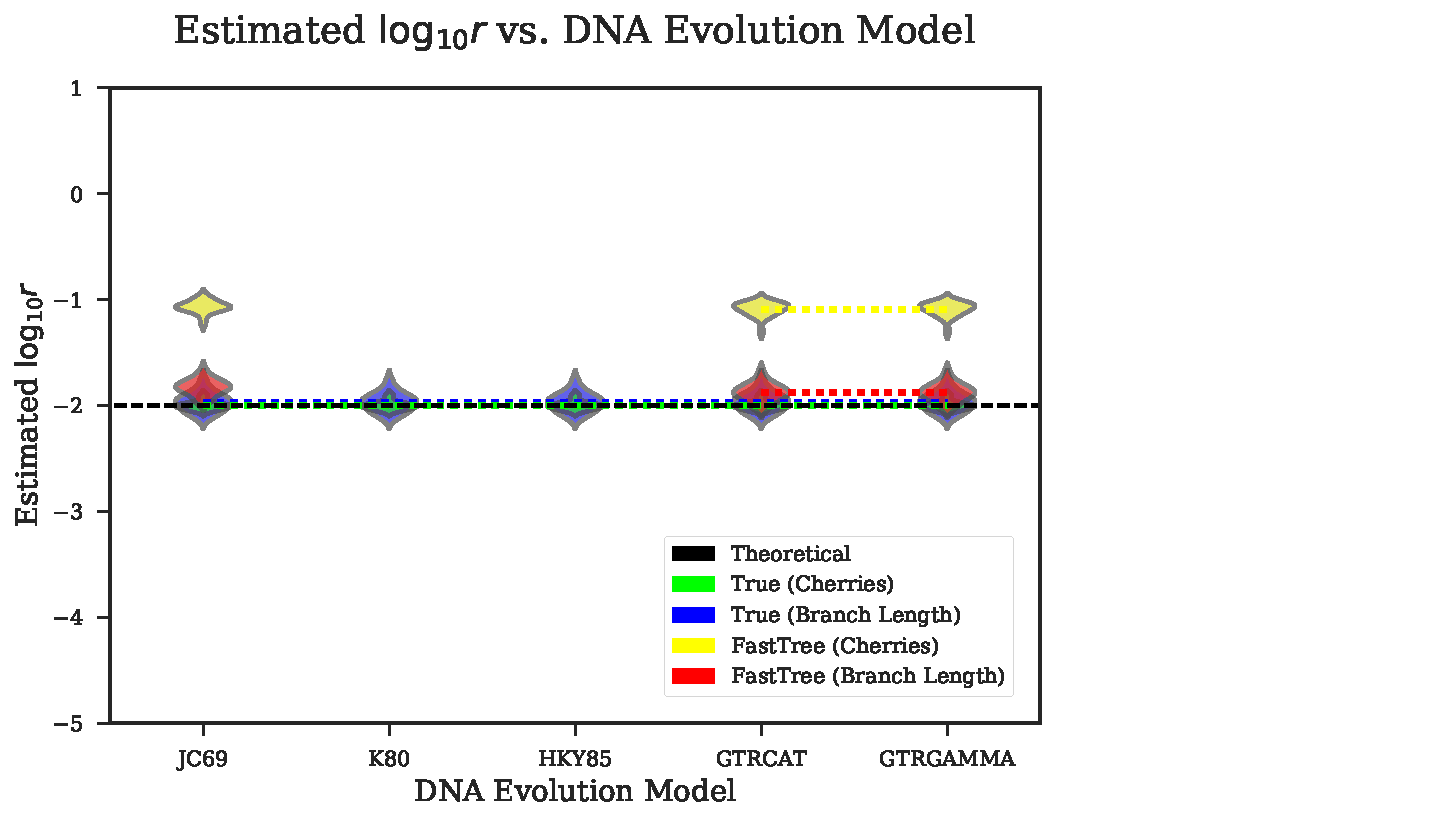
\includegraphics[width=0.3\textwidth]{figs/dualbirth-res-cherry-supp-b}
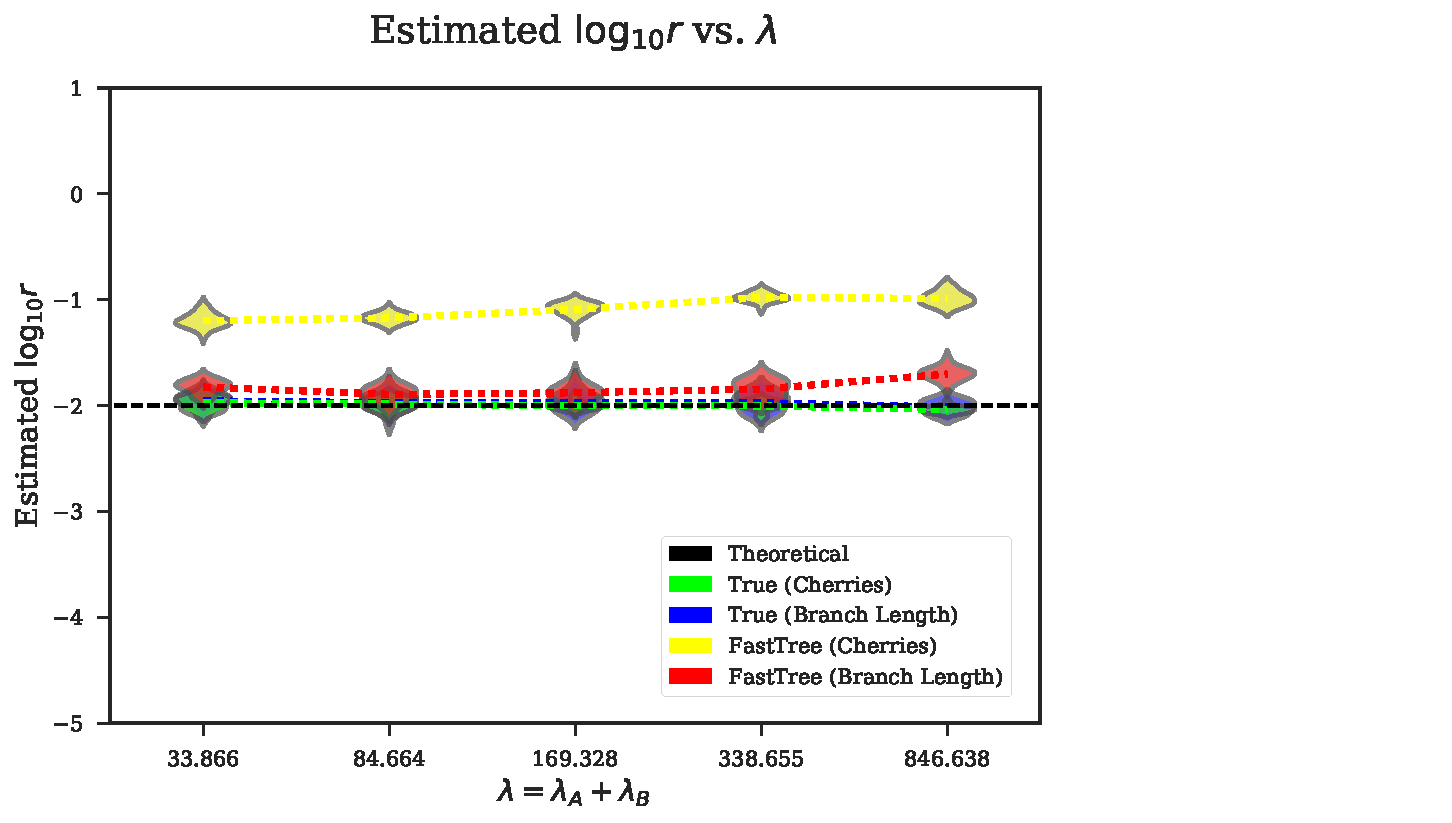
\includegraphics[width=0.3\textwidth]{figs/dualbirth-res-cherry-supp-c}\\
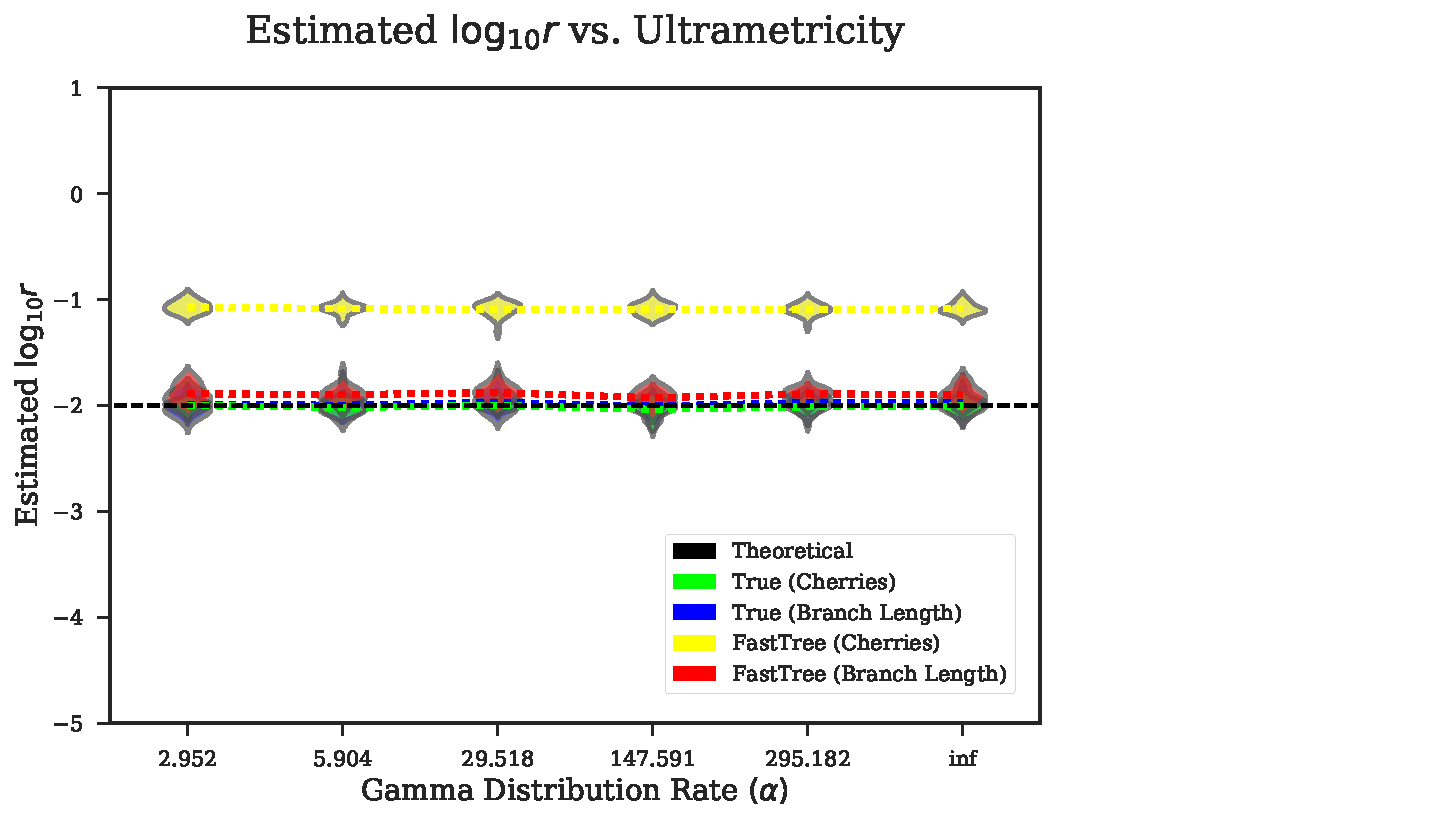
\includegraphics[width=0.3\textwidth]{figs/dualbirth-res-cherry-supp-d}
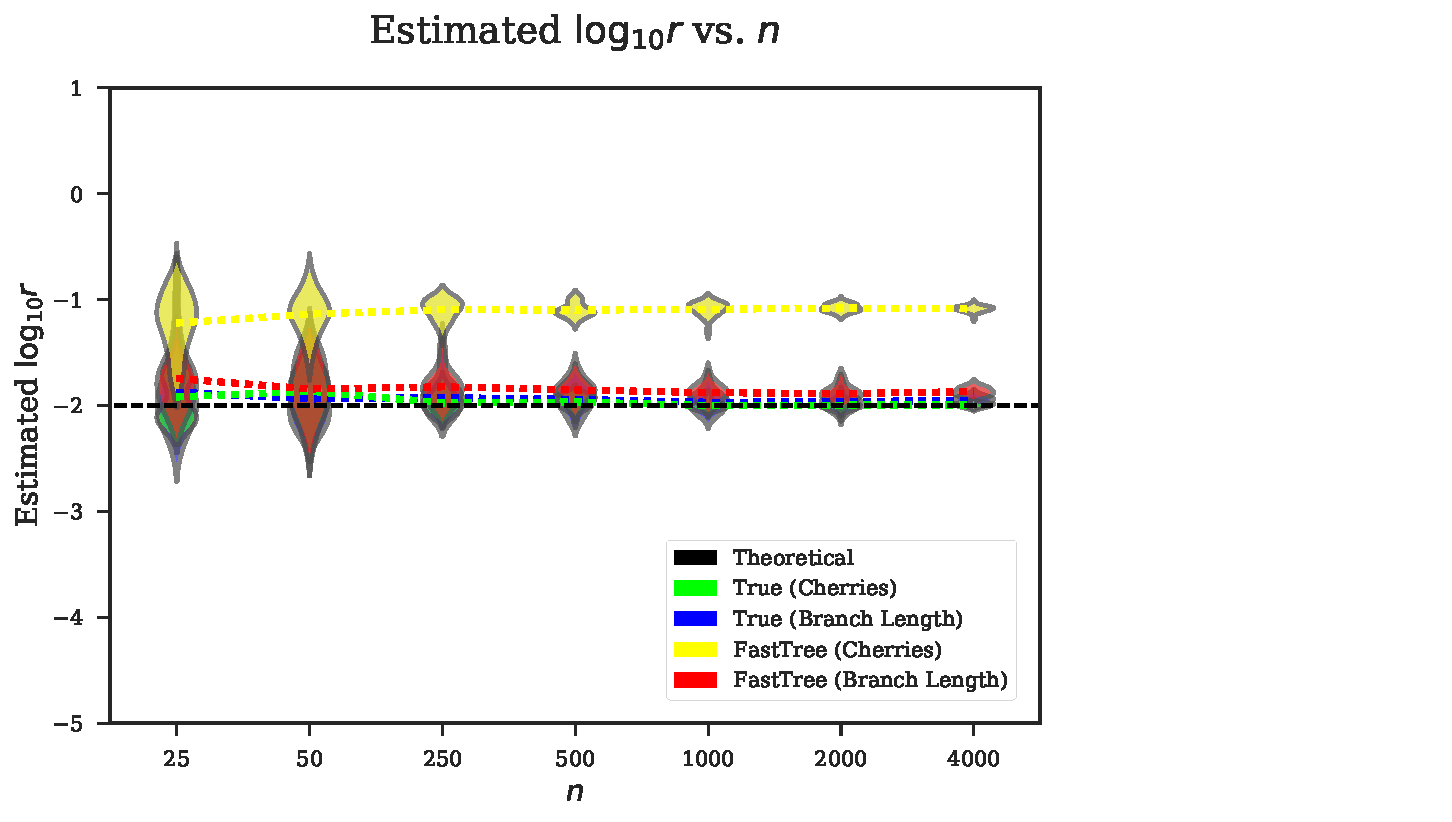
\includegraphics[width=0.3\textwidth]{figs/dualbirth-res-cherry-supp-e}
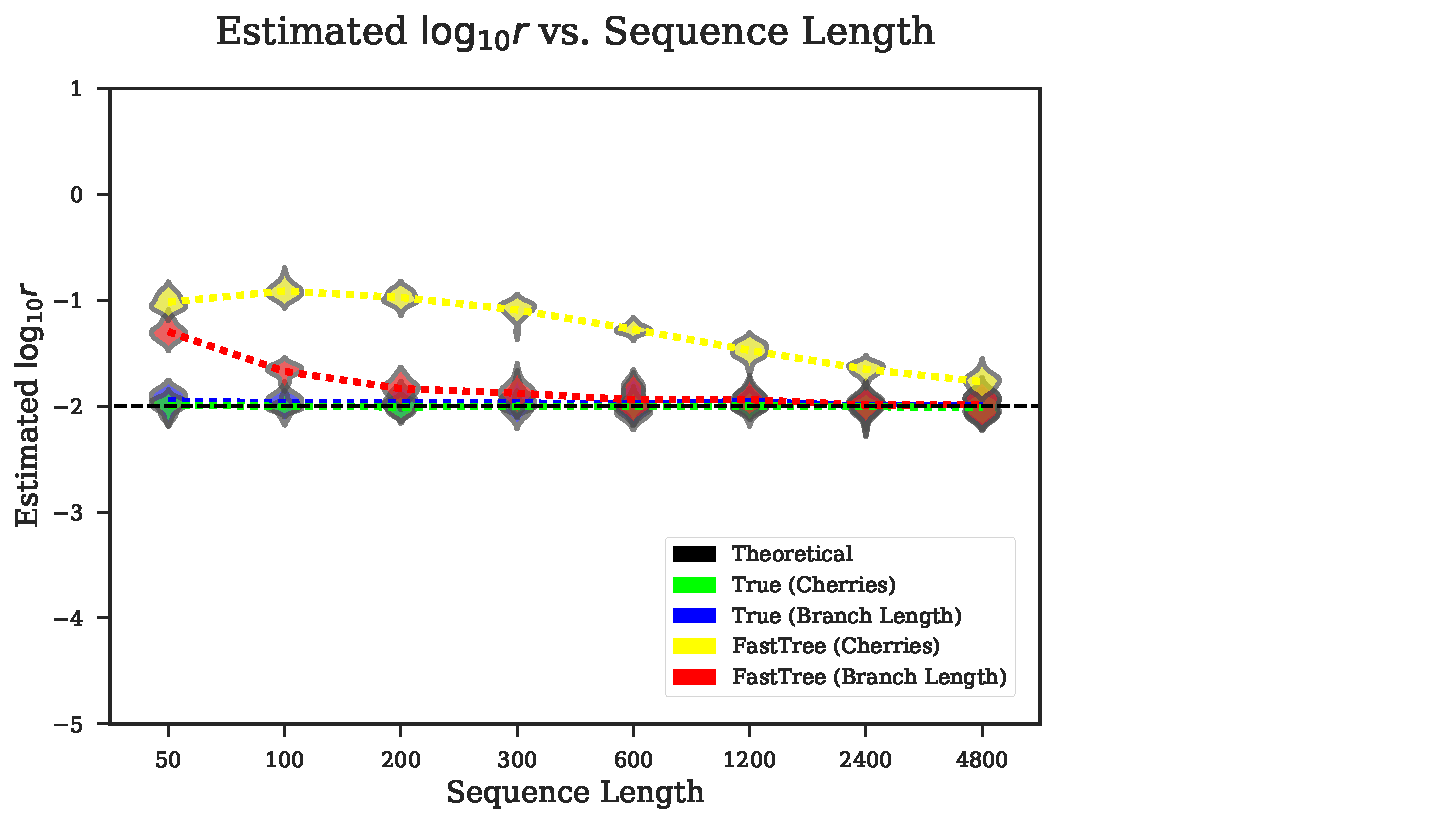
\includegraphics[width=0.3\textwidth]{figs/dualbirth-res-cherry-supp-f}
\caption[Parameter estimation accuracy]
{Parameter estimation accuracy. Violin plots are shown for the estimated $r$, using the cherry-based estimator and the branch-length-based estimator, for true trees and for inferred FastTree~2 trees for each of the experiments. Note that FastTree~2 does not have \gls{K80} or \gls{HKY85} models implemented.}
\label{fig:dualbirth-res-cherry-supp}
\end{figure}

\begin{figure} % FIGURE S12 IN ORIGINAL PAPER
\centering
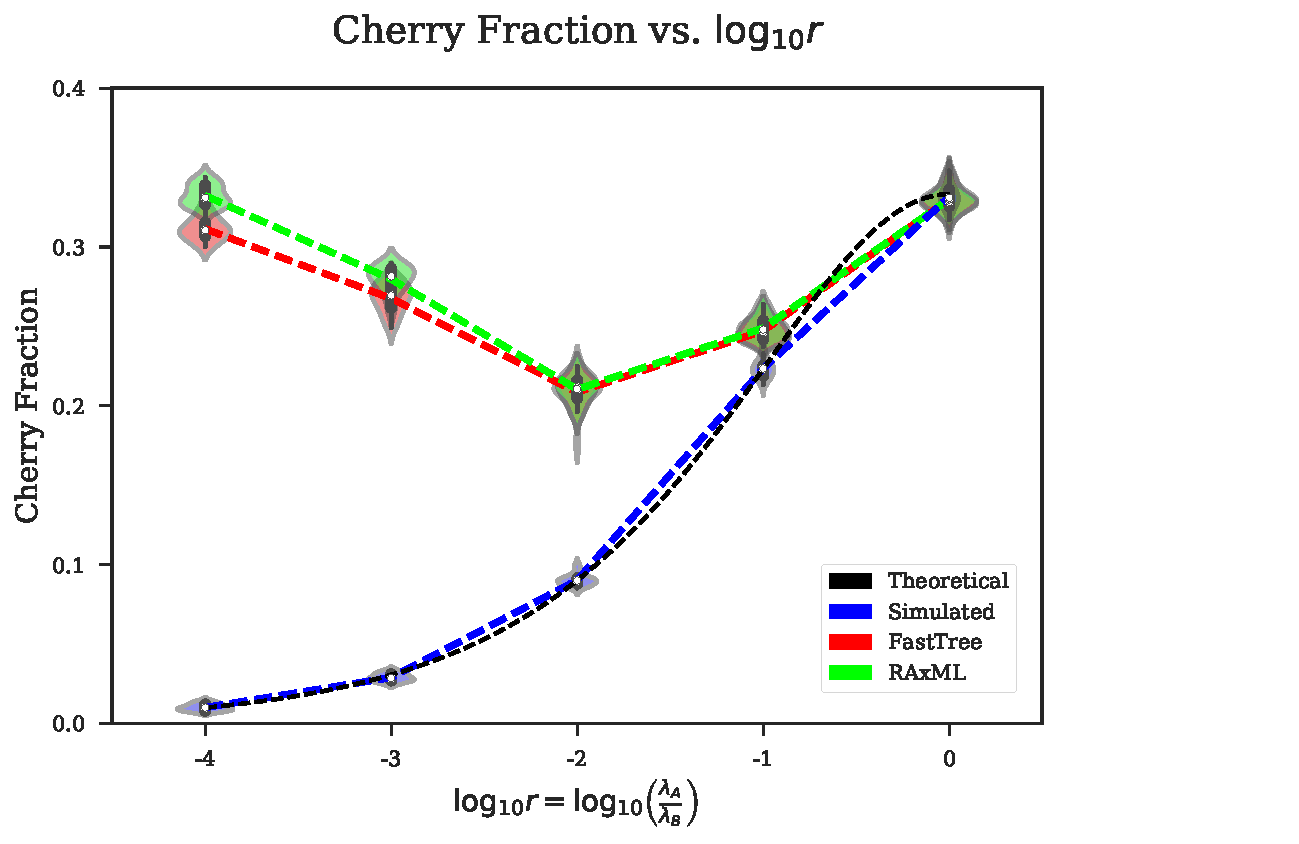
\includegraphics[width=0.3\textwidth]{figs/dualbirth-cherry-fraction-supp-a}
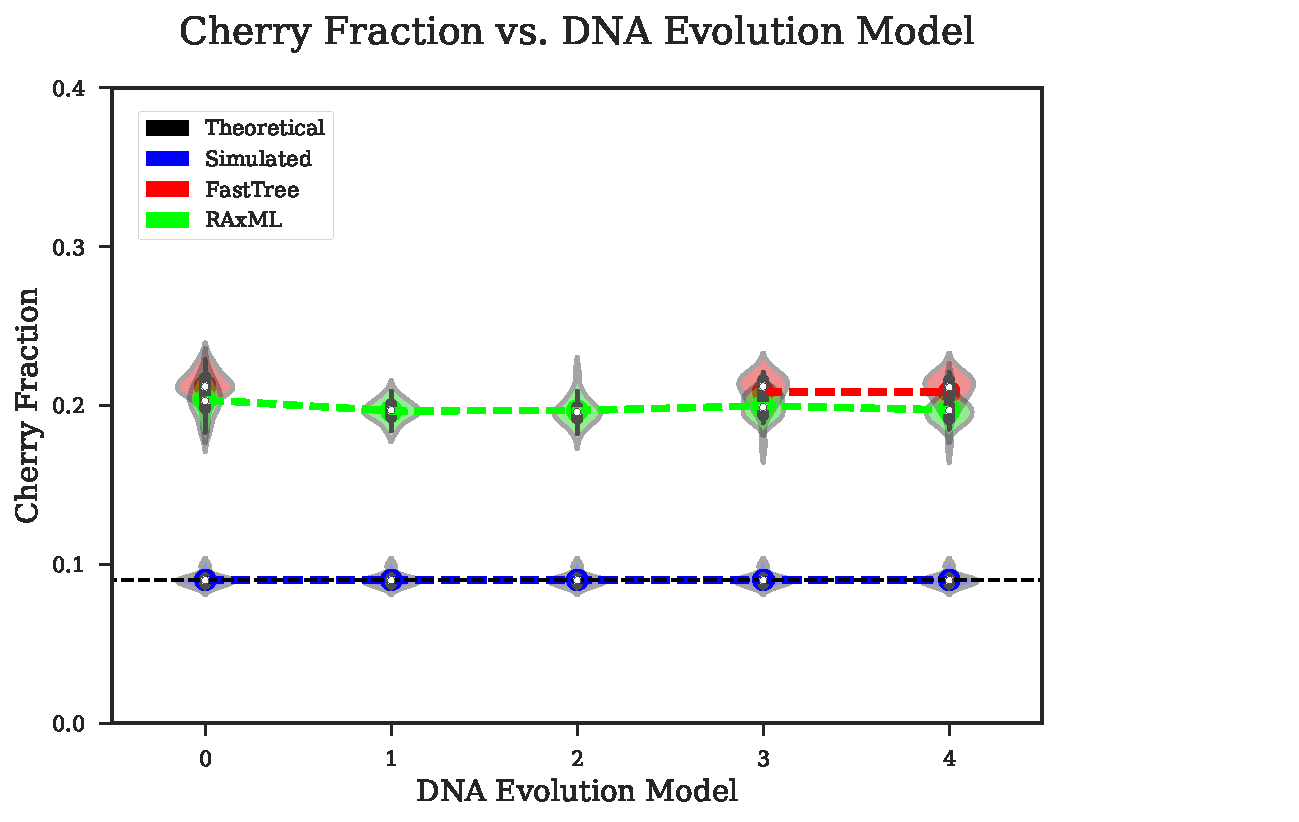
\includegraphics[width=0.3\textwidth]{figs/dualbirth-cherry-fraction-supp-b}
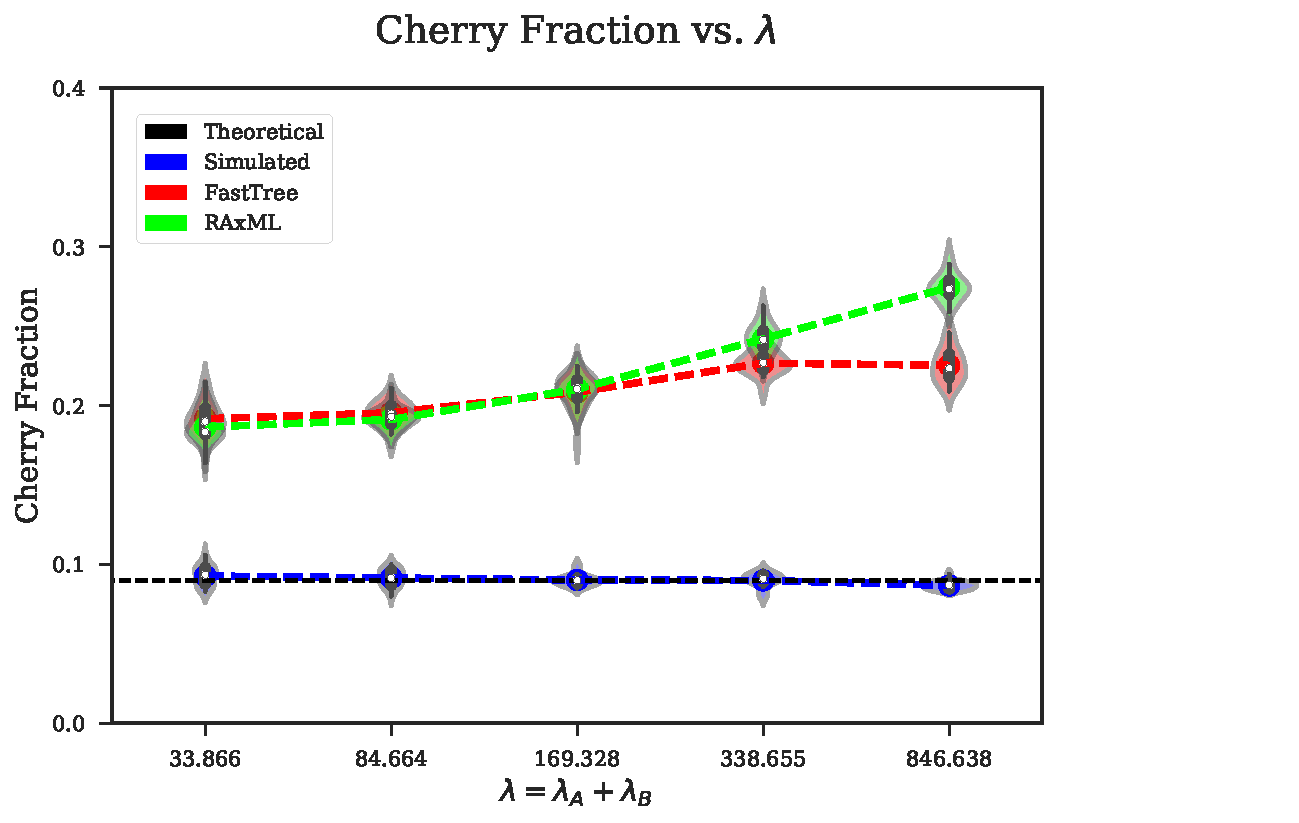
\includegraphics[width=0.3\textwidth]{figs/dualbirth-cherry-fraction-supp-c}\\
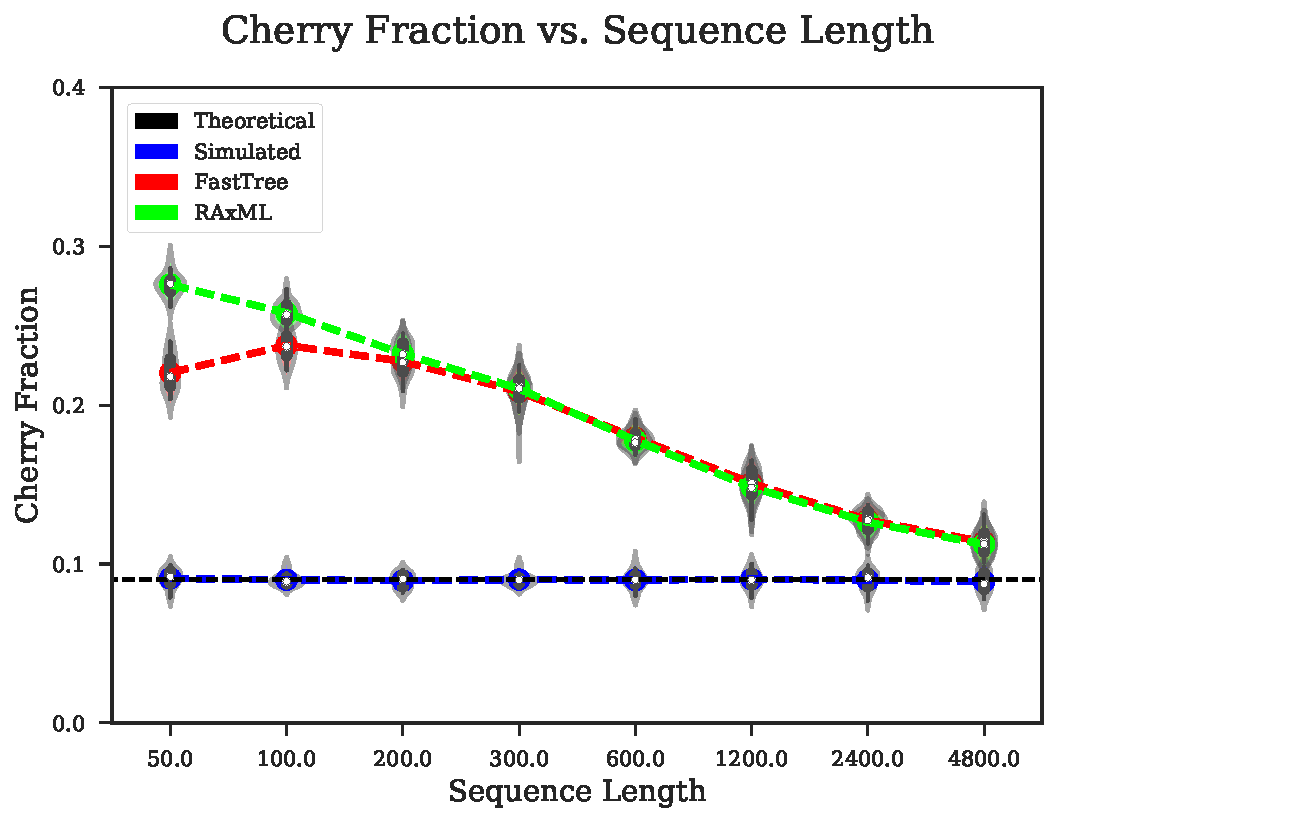
\includegraphics[width=0.3\textwidth]{figs/dualbirth-cherry-fraction-supp-d}
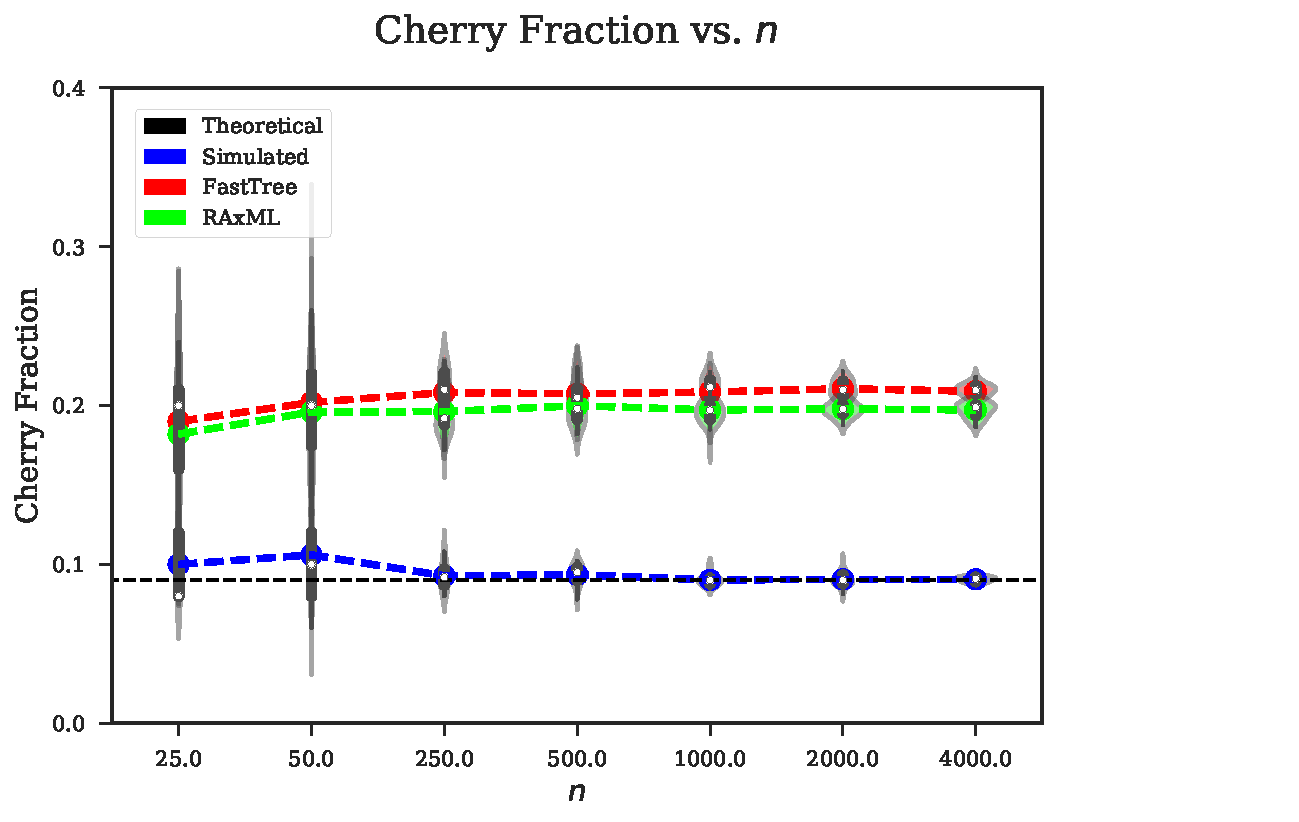
\includegraphics[width=0.3\textwidth]{figs/dualbirth-cherry-fraction-supp-e}
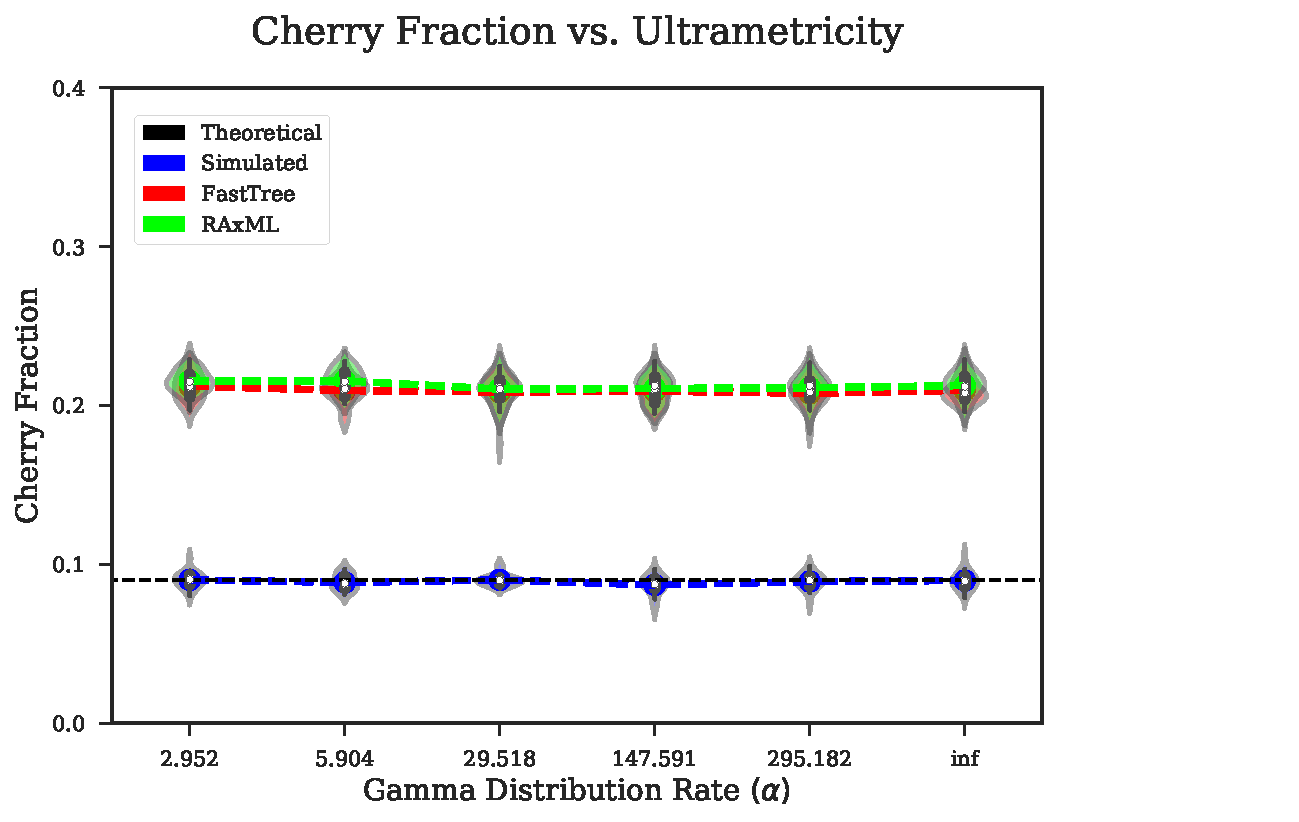
\includegraphics[width=0.3\textwidth]{figs/dualbirth-cherry-fraction-supp-f}
\caption[Cherry fraction]
{Cherry fraction. Violin plots are shown for the cherry fractions of the true trees and inferred RAxML and FastTree~2 trees.}
\label{fig:dualbirth-cherry-fraction-supp}
\end{figure}

\begin{figure} % FIGURE S13 IN ORIGINAL PAPER
\centering
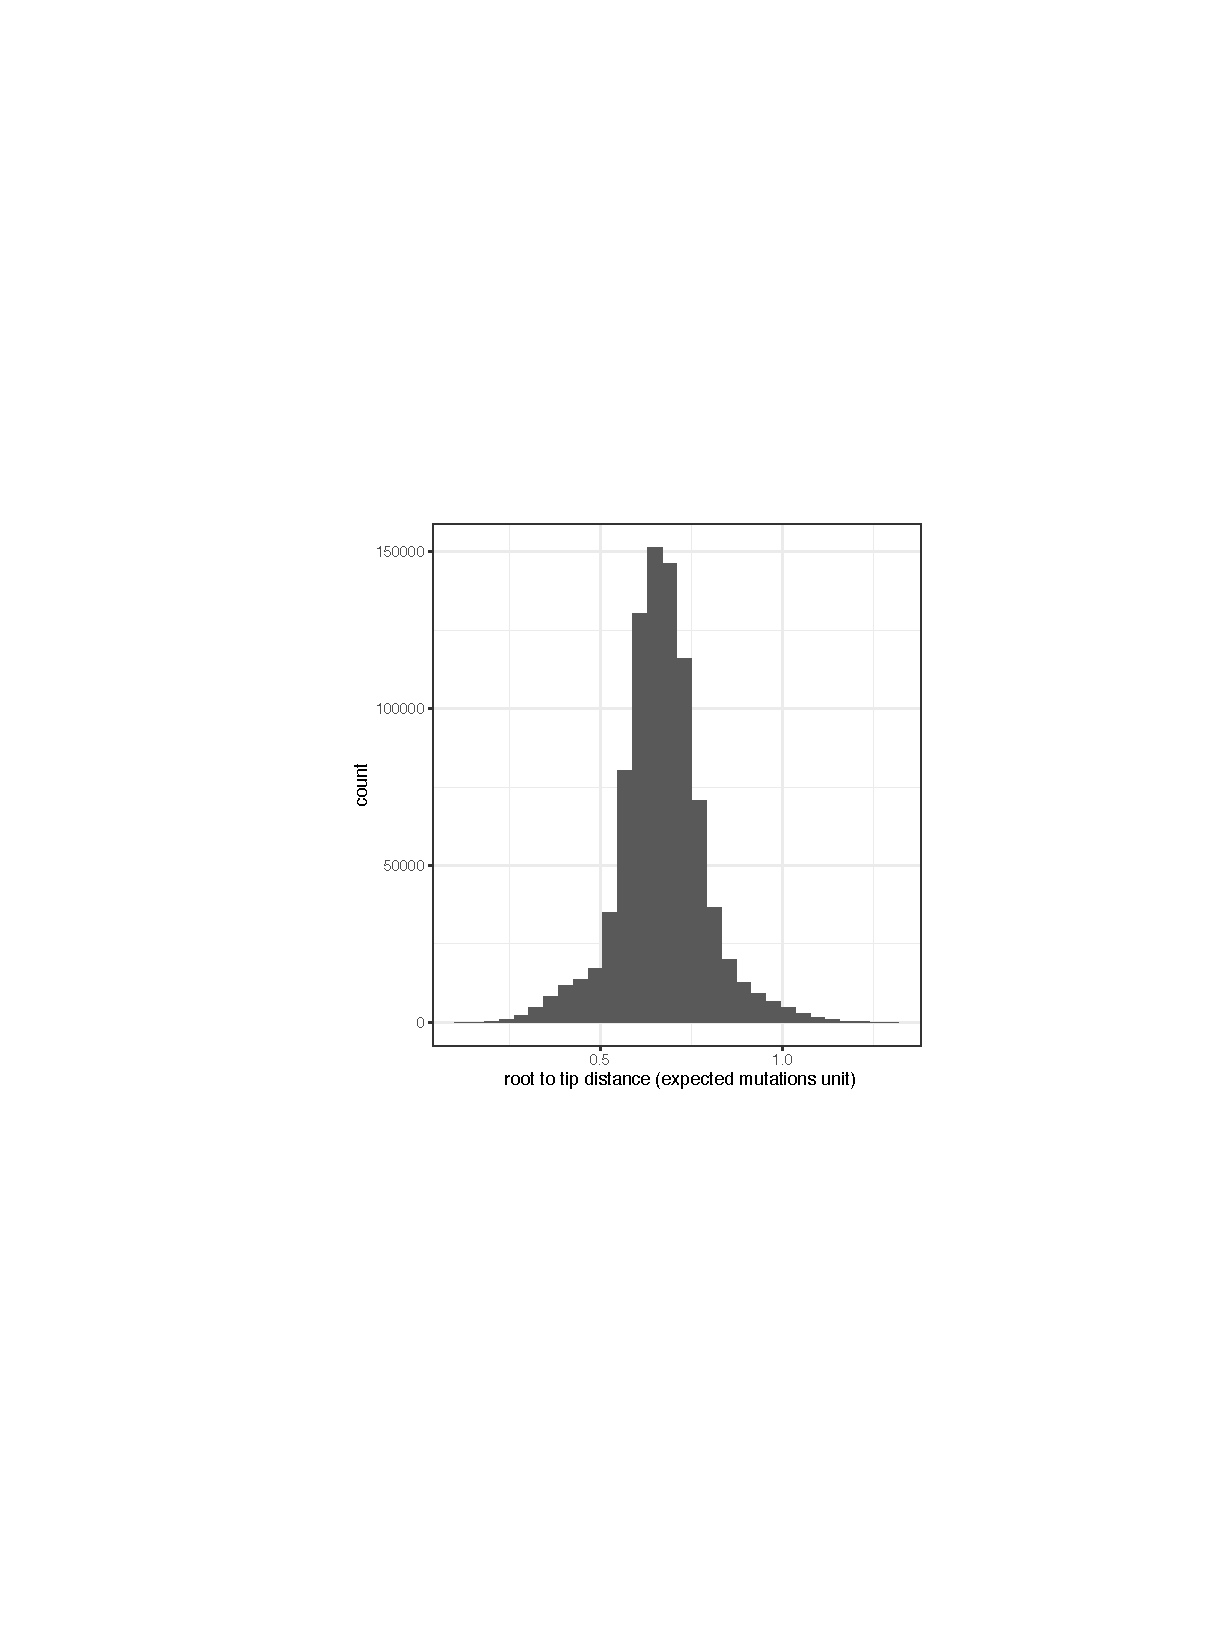
\includegraphics[width=0.8\textwidth]{figs/dualbirth-root-to-tip}
\caption[Molecular clock on the \textit{ Alu} tree]
{Molecular clock on the \textit{ Alu} tree. The distribution of the root-to-tip distances after midpoint rooting are shown for the \textit{ Alu} tree with 1\% masking. Under the molecular clock, root to tip distances for all leaves are expected to be identical.}
\label{fig:dualbirth-root-to-tip}
\end{figure}

%% END DUAL-BIRTH SUPPLEMENT